% Befehl \fibelvorstellung: Erstellt die Vorstellung eines FSlers mit Bild
%	Parameter #1: Bild (wrapfigure)
%	Parameter #2: Text
\newcommand{\fibelvorstellung}[2]{%
	\begin{minipage}{\columnwidth}
		% Kein Abstand vor bzw. nach Bildern bei wrapfigure
		\setlength{\intextsep}{0cm}
		% geringfügiger Abstand zwischen Paragraphen
		\setlength{\parskip}{0.5ex}
		#1
		#2
		\vspace{0.5ex}
	\end{minipage}
	
	\vspace{5ex plus 2ex minus 1ex}
}
\newlength{\fibelstdlen}
\setlength{\fibelstdlen}{3.7cm}

\section{Der Fachschaftsrat~(FSR) Physik stellt sich vor}
\begin{multicols*}{2}
\small
\fibelvorstellung{
	\begin{wrapfigure}{l}{0cm}
		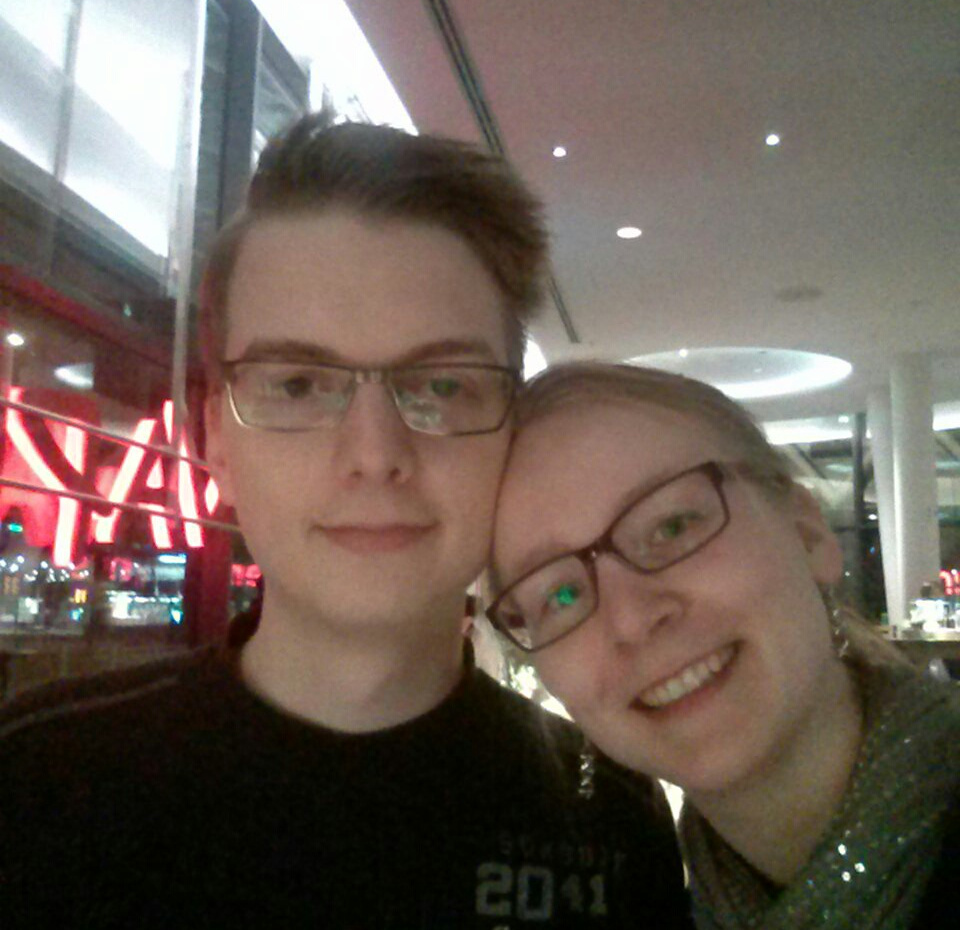
\includegraphics[width=5.1cm]{res/vorstellungsfotos/simon_may_alexandra_everwand_cropped.jpg}
	\end{wrapfigure}
}
{% LaTeX-Warnung deaktivieren
%\hbadness=10000

Hey,
ich bin Alex (rechts) und schon länger in der Fachschaft.  
Zur Zeit bin ich im Master und war ein Jahr in Schweden.
Dieses Jahr organisiere ich  die O-Woche, den Buchmarkt und bei den Spieleabenden helfe ich auch immer mit.
Fragt aber auch sonst ruhig nach, wenn ihr Hilfe braucht :-)
}

\fibelvorstellung{
	\begin{wrapfigure}{r}{0cm}
		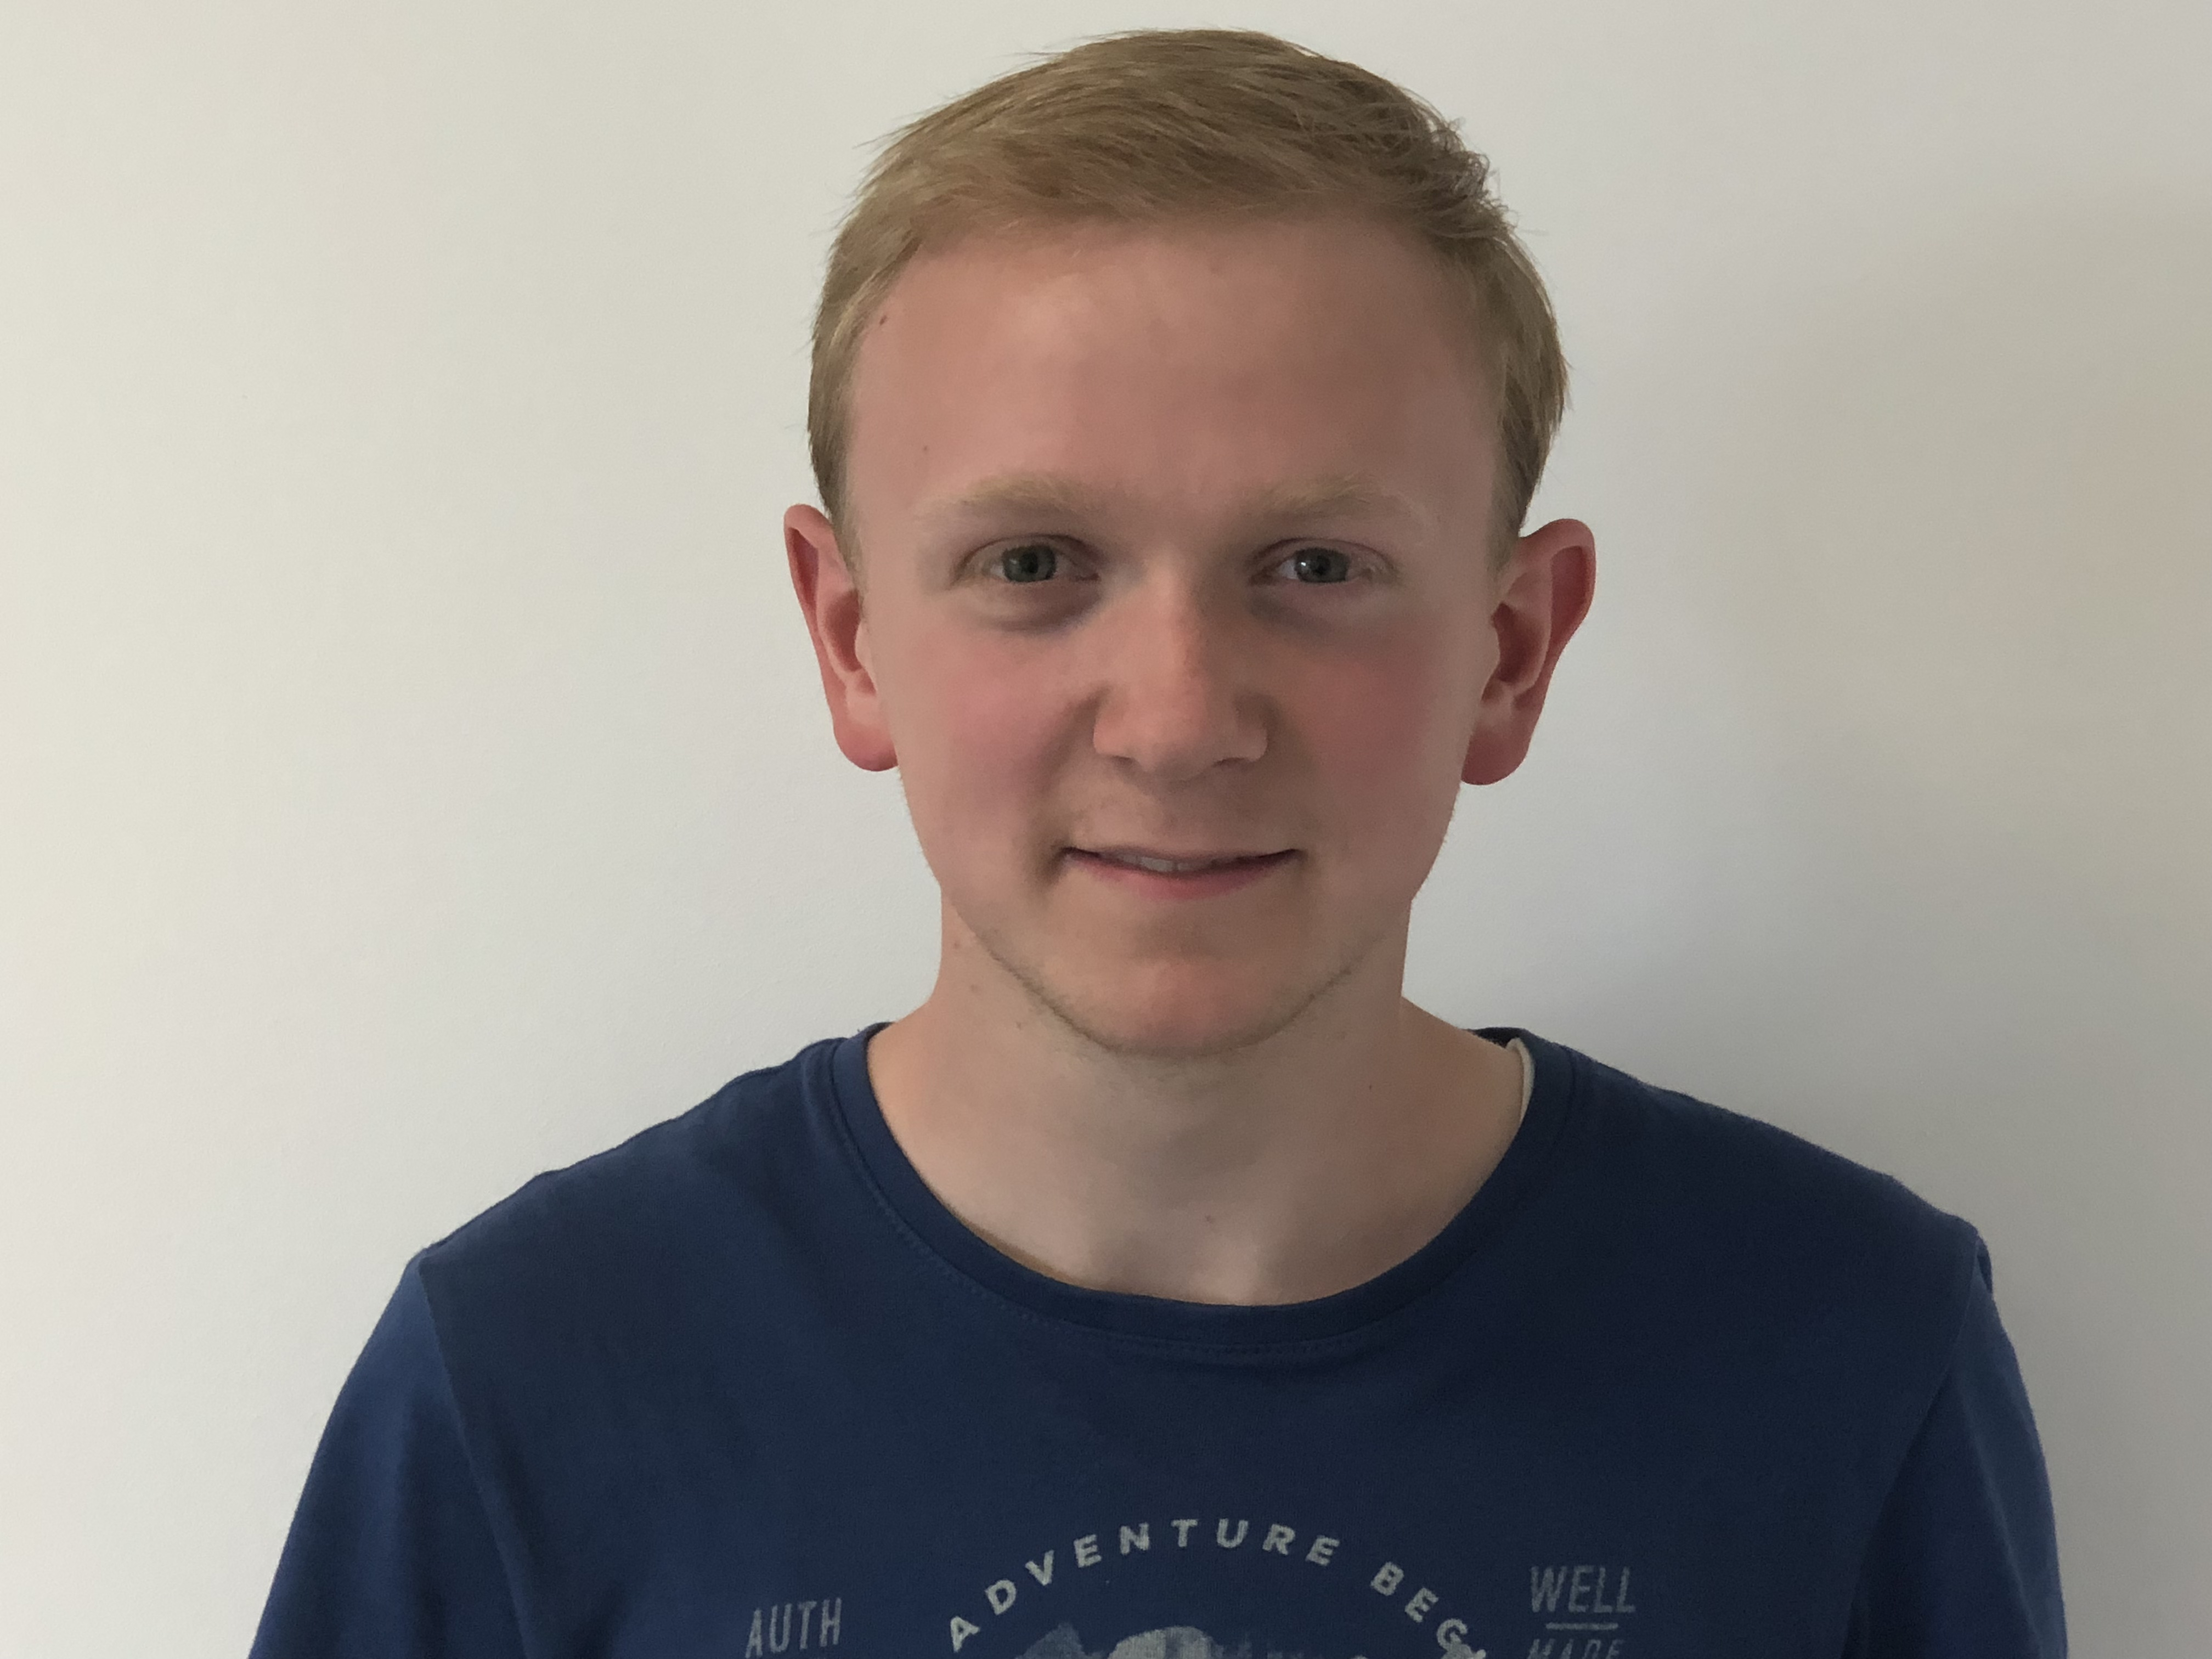
\includegraphics[width=\fibelstdlen]{res/vorstellungsfotos/tim_stellhorn.JPG}
	\end{wrapfigure}
}
{Hey Leute, ich bin Tim und studiere seit 2 Semestern Physik mit Nebenfach Informatik. Ich kann euch nur sagen, lasst euch auf keinen Fall von einem vielleicht etwas schwierigen Einstieg verunsichern, das wird schon. Doch erstmal möchte ich euch noch viel Spaß in der O-Woche wünschen. Und wenn ihr Lust habt, dann schaut mal beim Spieleabend der Fachschaft vorbei, vielleicht sieht man sich da ja wieder ;-)}

\fibelvorstellung{
	\begin{wrapfigure}{l}{0cm}
		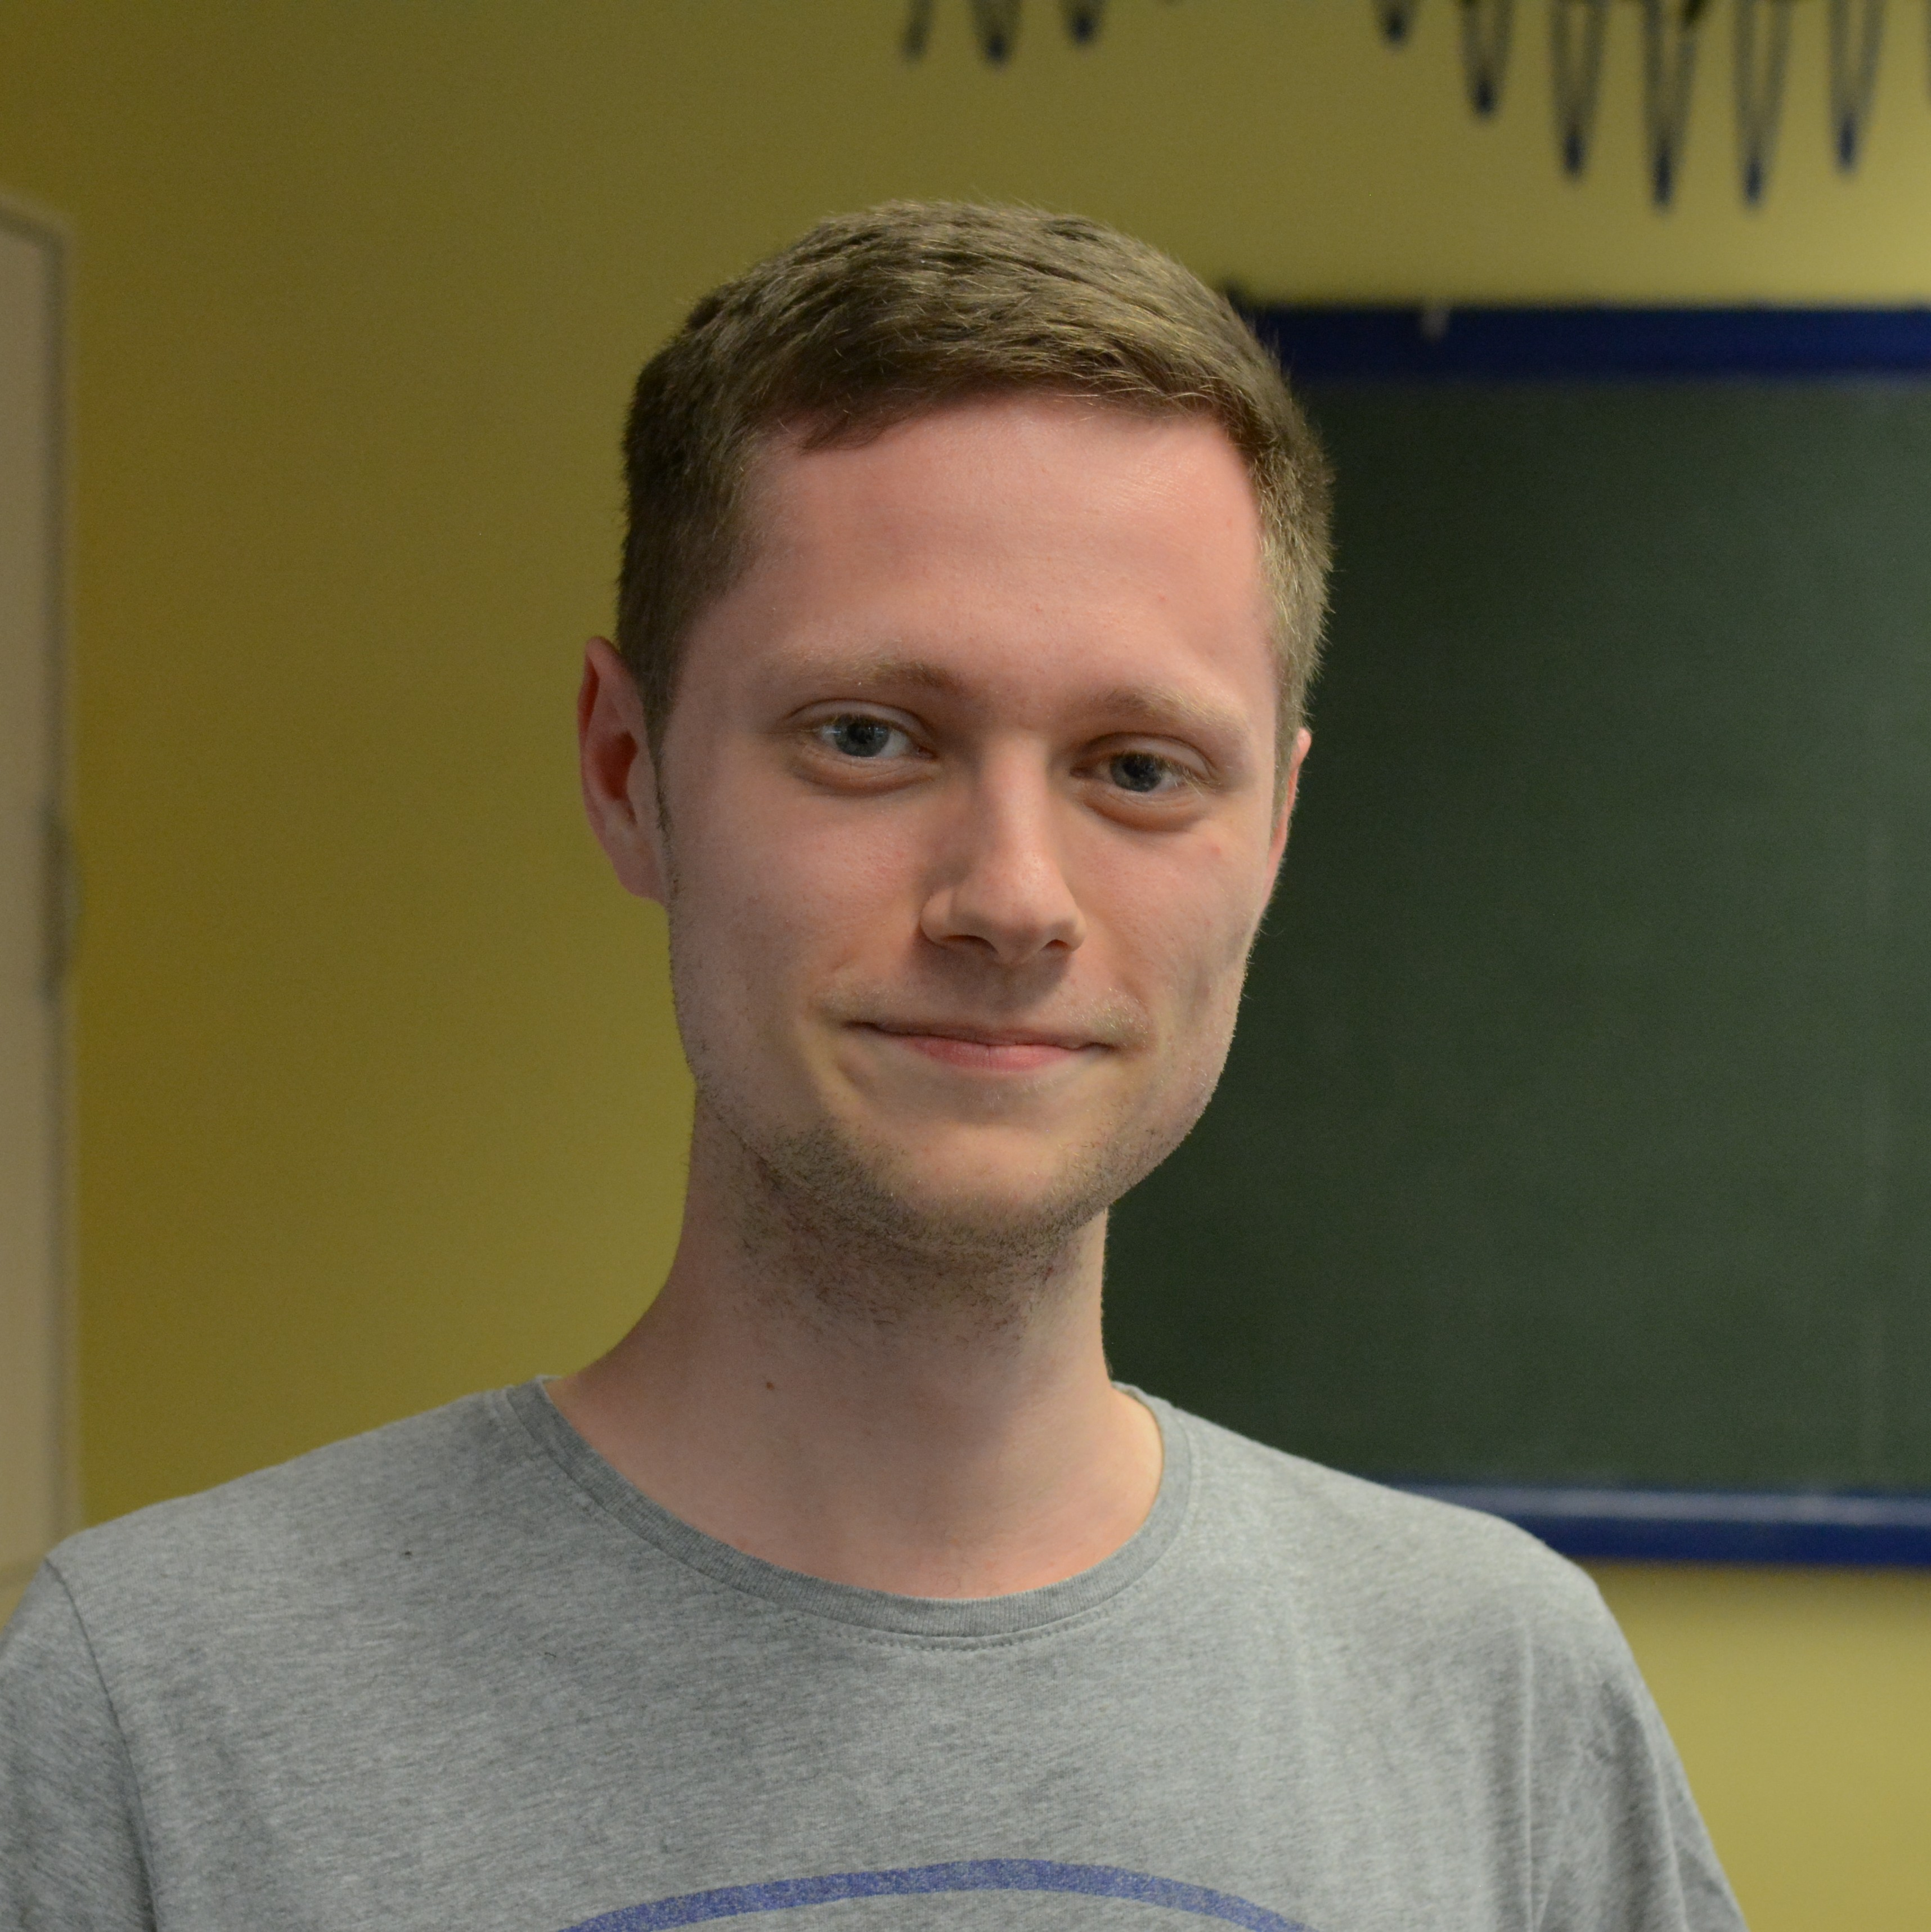
\includegraphics[width=\fibelstdlen]{res/vorstellungsfotos/carsten_staab.JPG}
	\end{wrapfigure}
}
{Servus! Ich bin der Carsten, studiere den B.Sc. Physik im 3. Semester und bin fast seit dem ersten Tag in der Fachschaft. Denkt immer dran: Es gibt keine dummen Fragen. Also, wenn ihr was wissen wollt, fragt einfach drauf los!
}	


\fibelvorstellung{
	\begin{wrapfigure}{r}{0cm}
		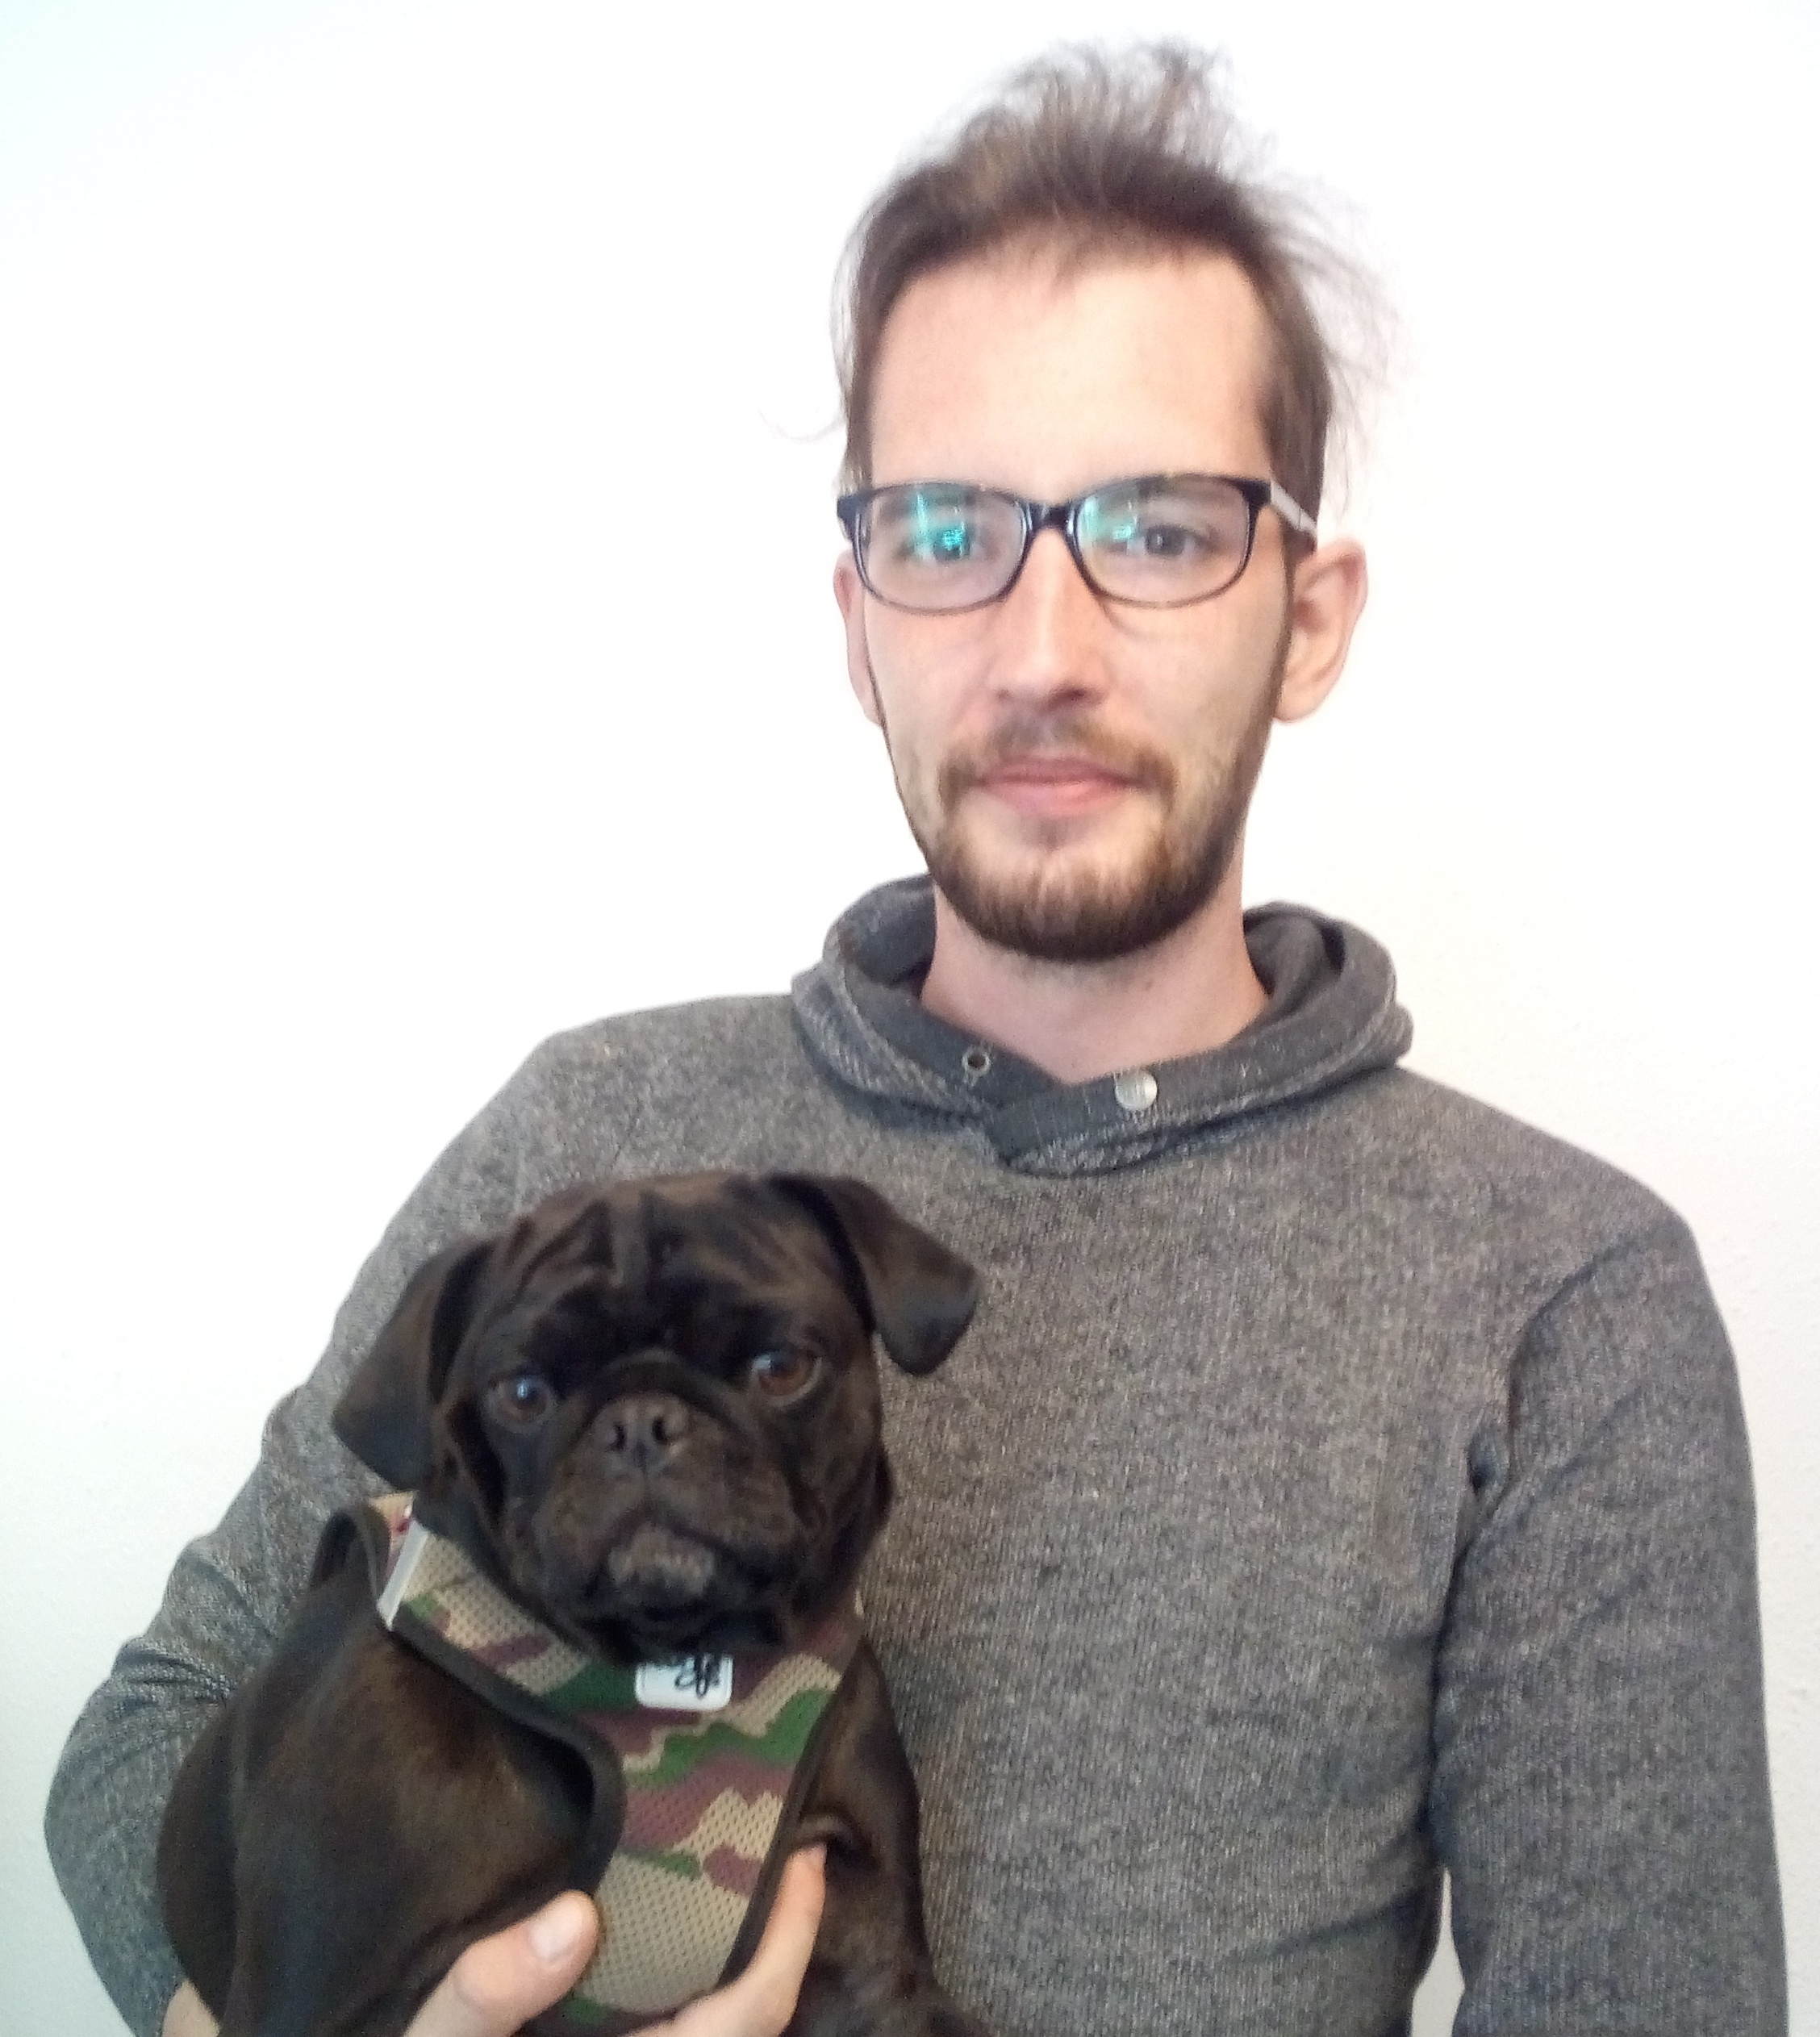
\includegraphics[width=\fibelstdlen]{res/vorstellungsfotos/Hansi_Rutherford_cropped.jpg}
	\end{wrapfigure}
}
{Hallo, wir sind Hansi und Einstein. Ich (Hansi, nicht Einstein) bin hauptsächlich für die Evaluation zuständig, außerdem bin ich im O-Wochenteam. 
	Willkommen an der WWU}
\vspace{0.5cm}


\fibelvorstellung{
	\begin{wrapfigure}{l}{0cm}
		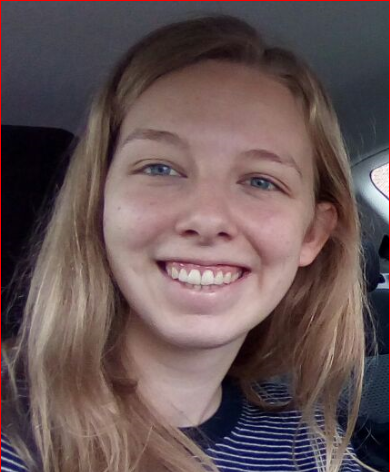
\includegraphics[width=\fibelstdlen]{res/vorstellungsfotos/anna_niemann_cropped.PNG}
	\end{wrapfigure}
}
{Hey, ich heiße Anna. Mit Fragen zum Studium oder Rund um Münster könnt ihr euch
	natürlich auch gerne an mich wenden. Ansonsten wünsche ich euch erstmal einen guten
	Start ins Studium:)
}
\vspace{0.5cm}

\fibelvorstellung{
	\begin{wrapfigure}{r}{0cm}
		\includegraphics[width=\fibelstdlen]{res/vorstellungsfotos/benedikt_bieringer.png}
	\end{wrapfigure}
}
{Hallo zusammen! Mein Name ist Benedikt. In der Fachschaft beschäftige ich mich unter anderem mit Computergrafik/Design. Programmieren und Schwimmen sind nur zwei meiner weiteren Freizeitbeschäftigungen. In meinen mittlerweile schon 8~Semestern Fachschafts- und Studienerfahrung kann ich euch aber auch bei einer ganzen Reihe weiterer Fragen weiterhelfen. 
}
\vspace{0.5cm}


\fibelvorstellung{
	\begin{wrapfigure}{l}{0cm}
		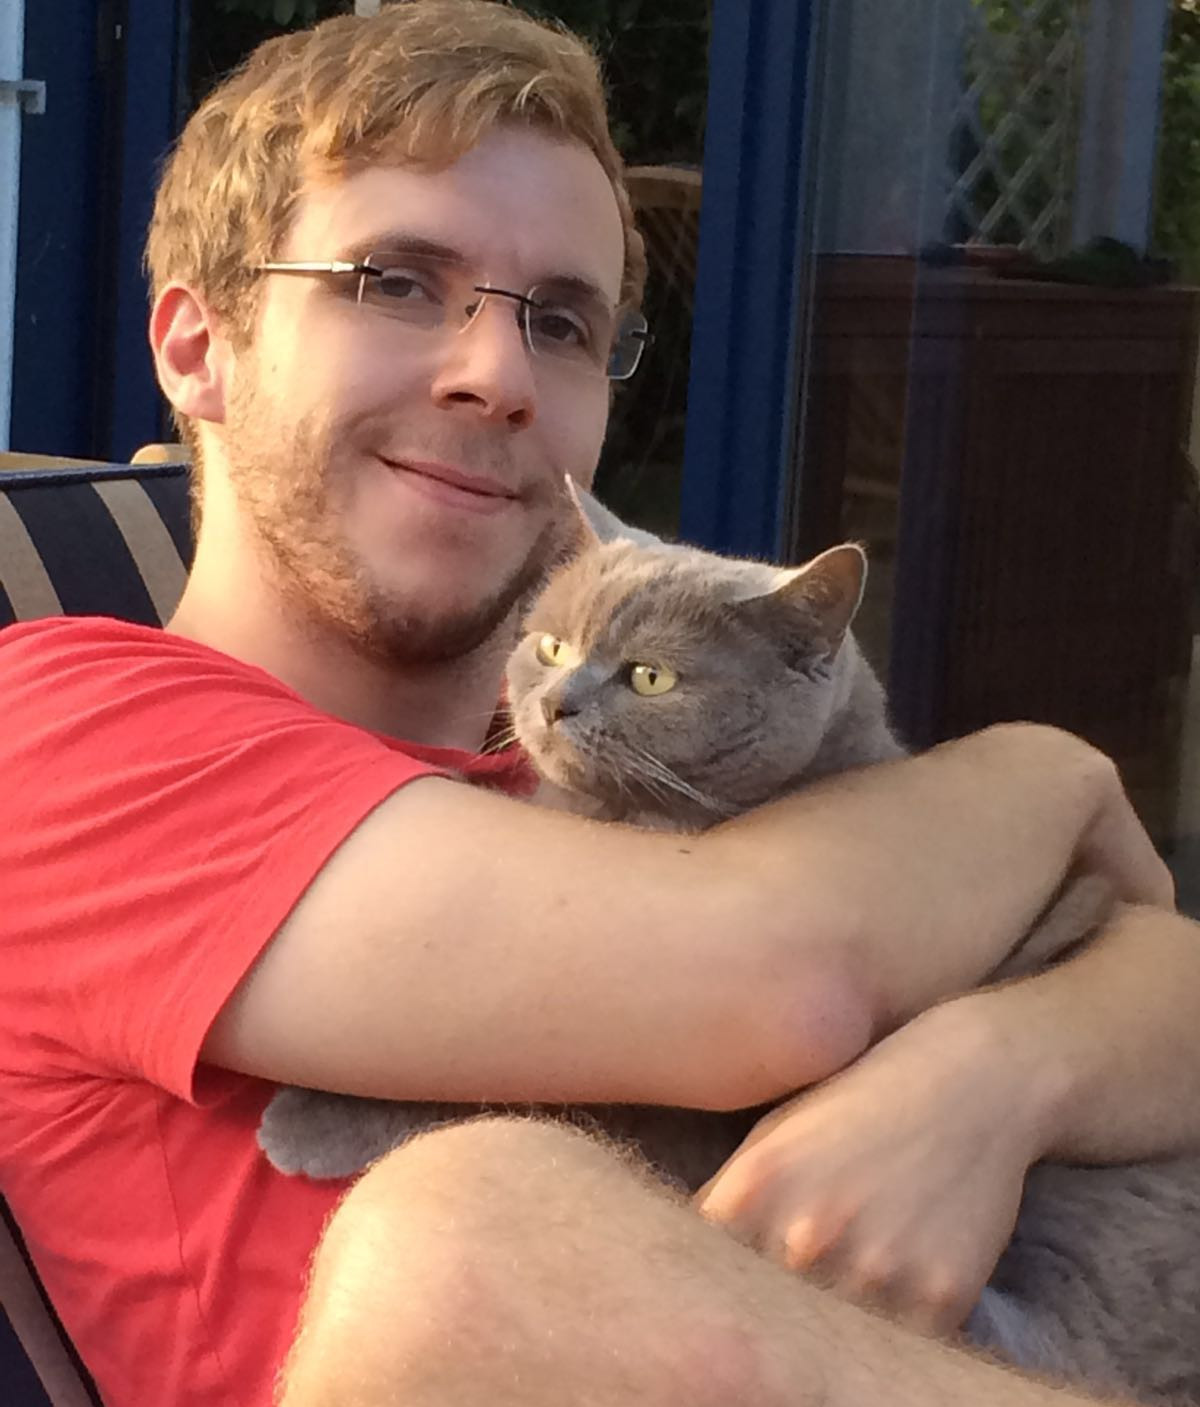
\includegraphics[width=\fibelstdlen]{res/vorstellungsfotos/lukas_eschmann_cropped.jpg}
	\end{wrapfigure}
}
{Moin liebe Erstis,
	mein Name ist Lukas und schon seit 2012 in der Fachschaft. Mein "normales" Studium habe ich bereits abgeschlossen, kann also so ziemlich alle Fragen zum Studium beantworten.
	Ich bin mittlerweile im Promotionsstudiengang angekommen und bin nur noch wenig in Hörsälen oder dem Fachschaftsraum anzutreffen.
	Auch Fragen zu Forschungsschwerpunkten der Uni oder aktuellen Themen der Forschung könnt ihr mir gerne stellen.}



\fibelvorstellung{
	\begin{wrapfigure}{r}{0cm}
		\includegraphics[width=\fibelstdlen]{res/vorstellungsfotos/philip_render_cropped.png}
	\end{wrapfigure}
}
{Hi, ich bin der Philip. Bin schon ein bisschen länger an der Uni und oft an der charakteristischen Bierpulle zu erkennen ;)
	
	Als 2FB kann ich euch auch übrigens immer gut von den schönen Seiten des Physikstudiums berichten.
	\vspace{\baselineskip}}


\fibelvorstellung{
	\begin{wrapfigure}{l}{0cm}
		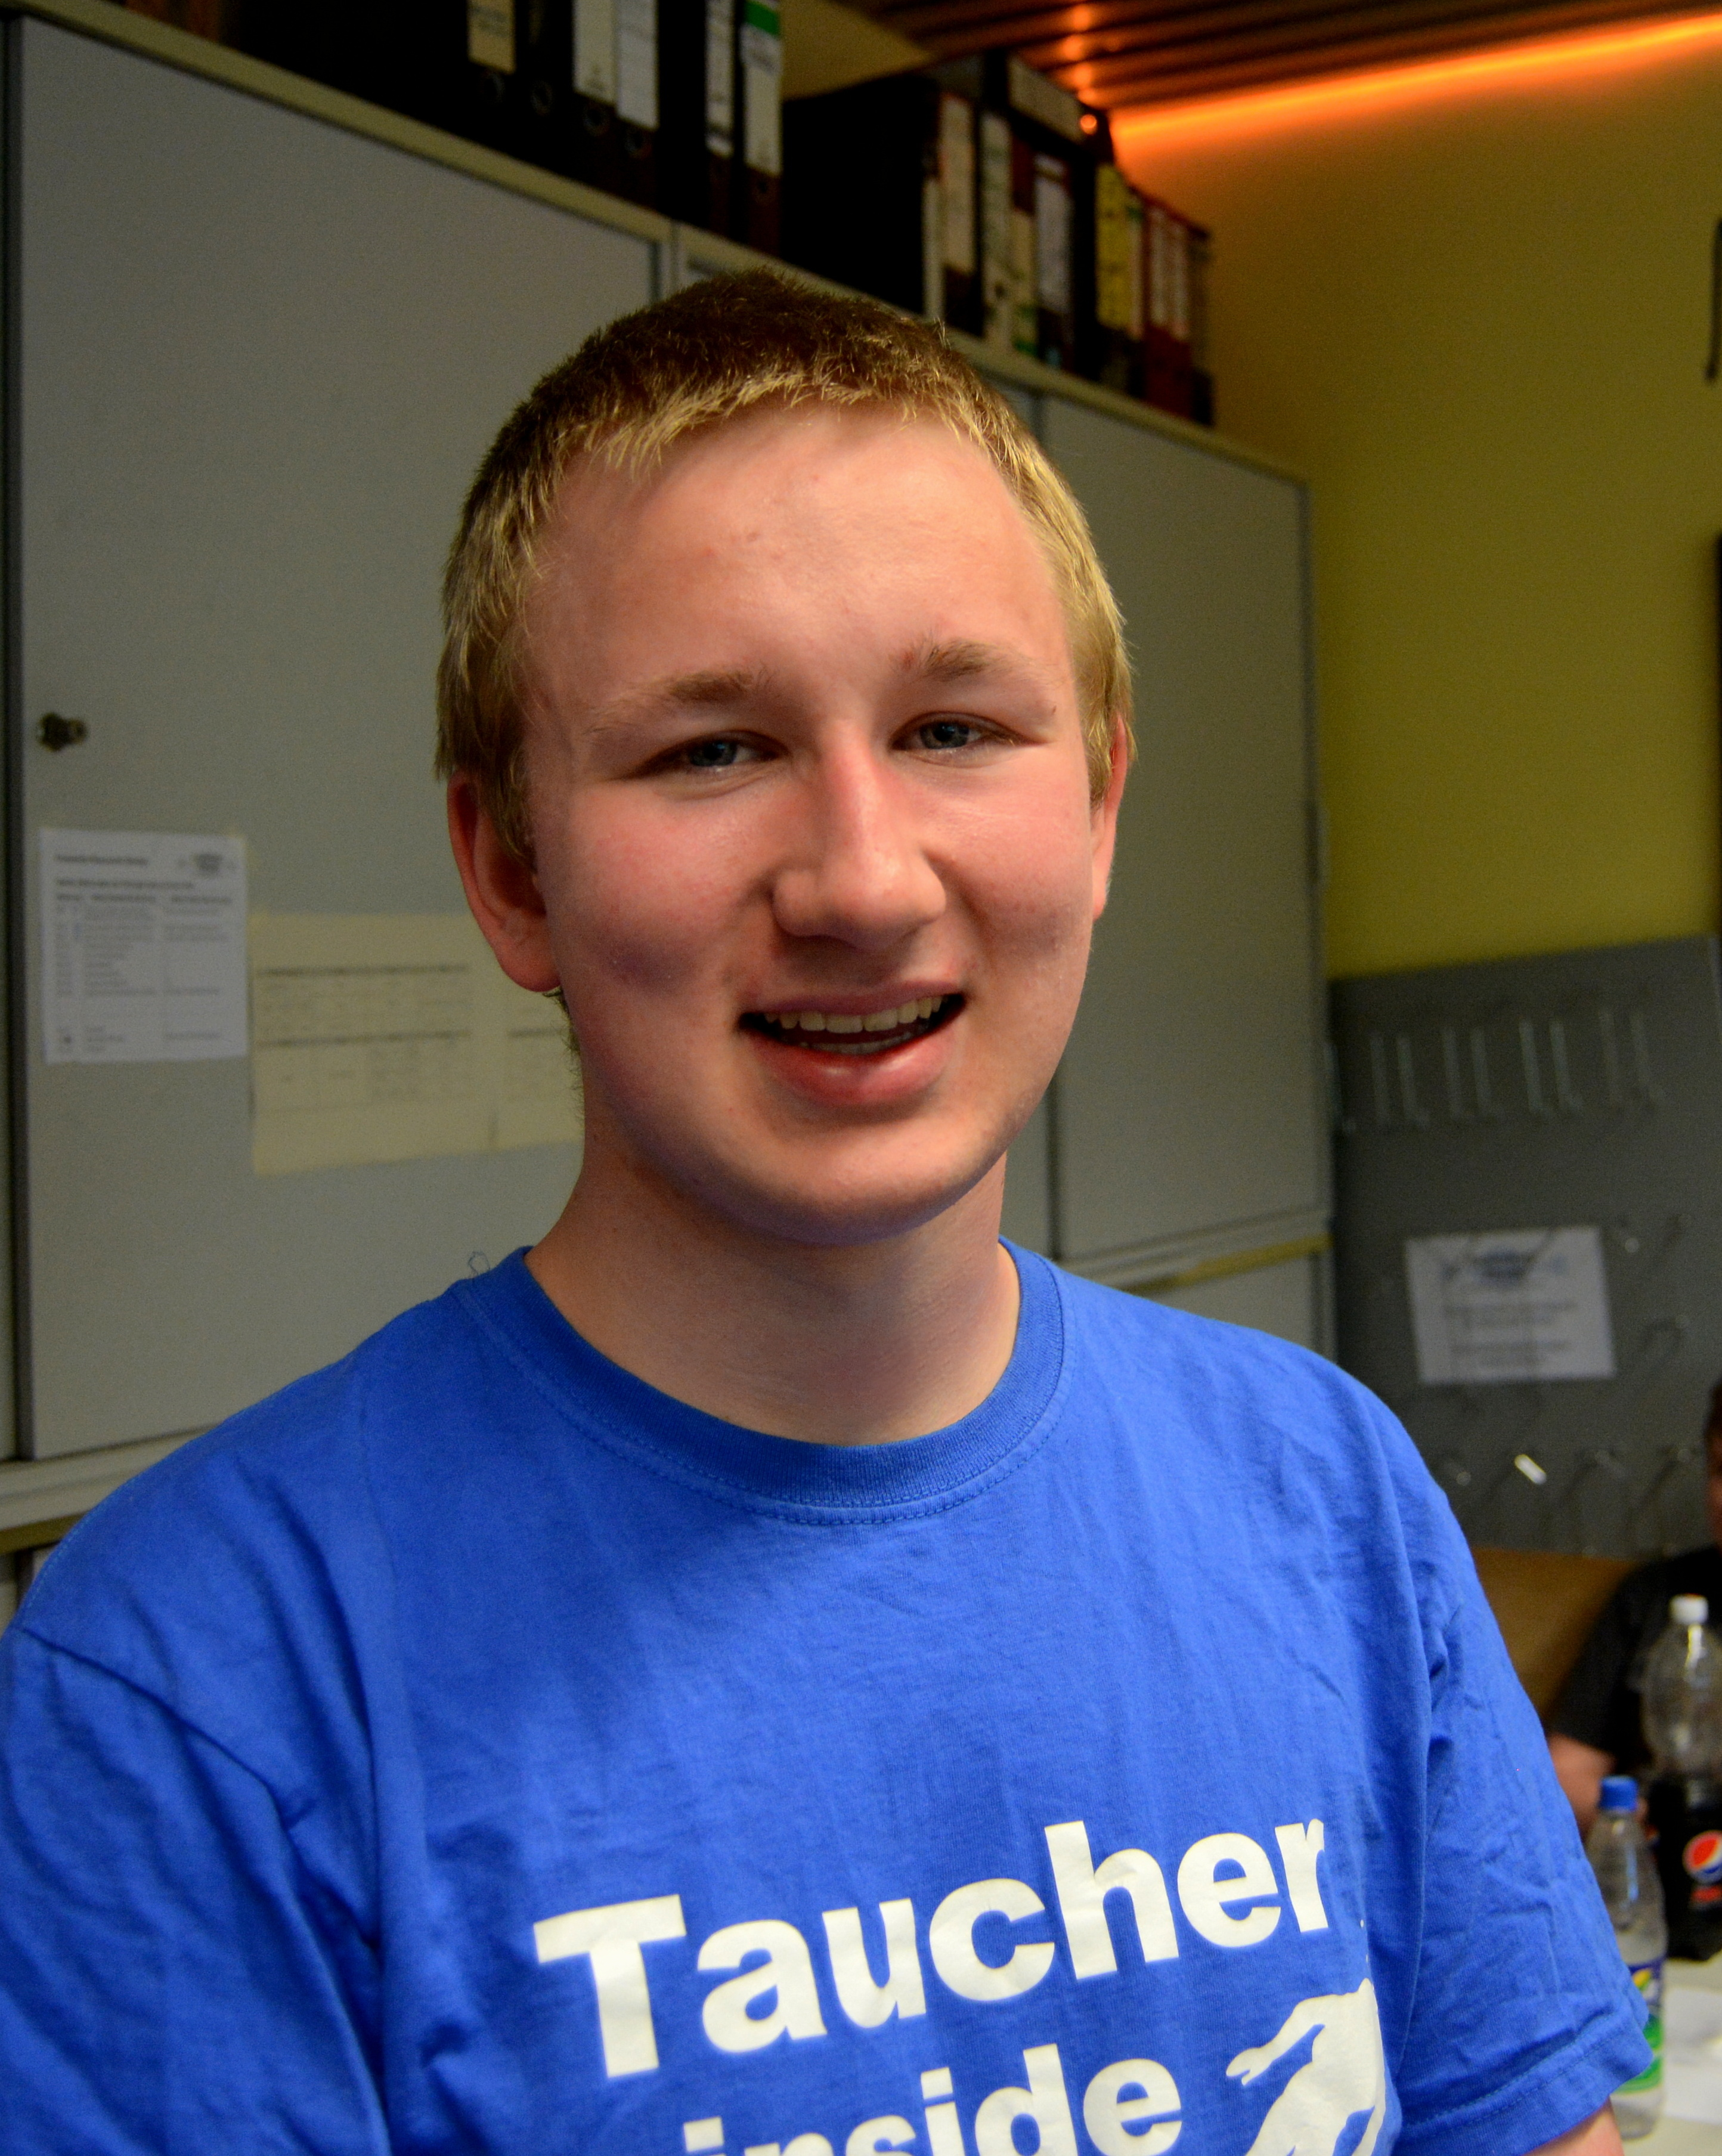
\includegraphics[width=\fibelstdlen]{res/vorstellungsfotos/hauke_hawighorst_cropped.jpg}
	\end{wrapfigure}
}
{Moin, ich bin Hauke und seit dem Ws16/17 an der Uni und in der Fachschaft.
In den letzten Jahren habe ich mich um die Evaluation der Lehrveranstaltungen gekümmert. Dieses Jahr werde ich als Erasmusstudent in Sevilla verbringen, danach stehe ich wieder der Fachschaft zur Verfügung. An euch ein herzliches Willkommen in Münster! 
	\vspace{2\baselineskip}
}

\fibelvorstellung{
	\begin{wrapfigure}{l}{0cm}
		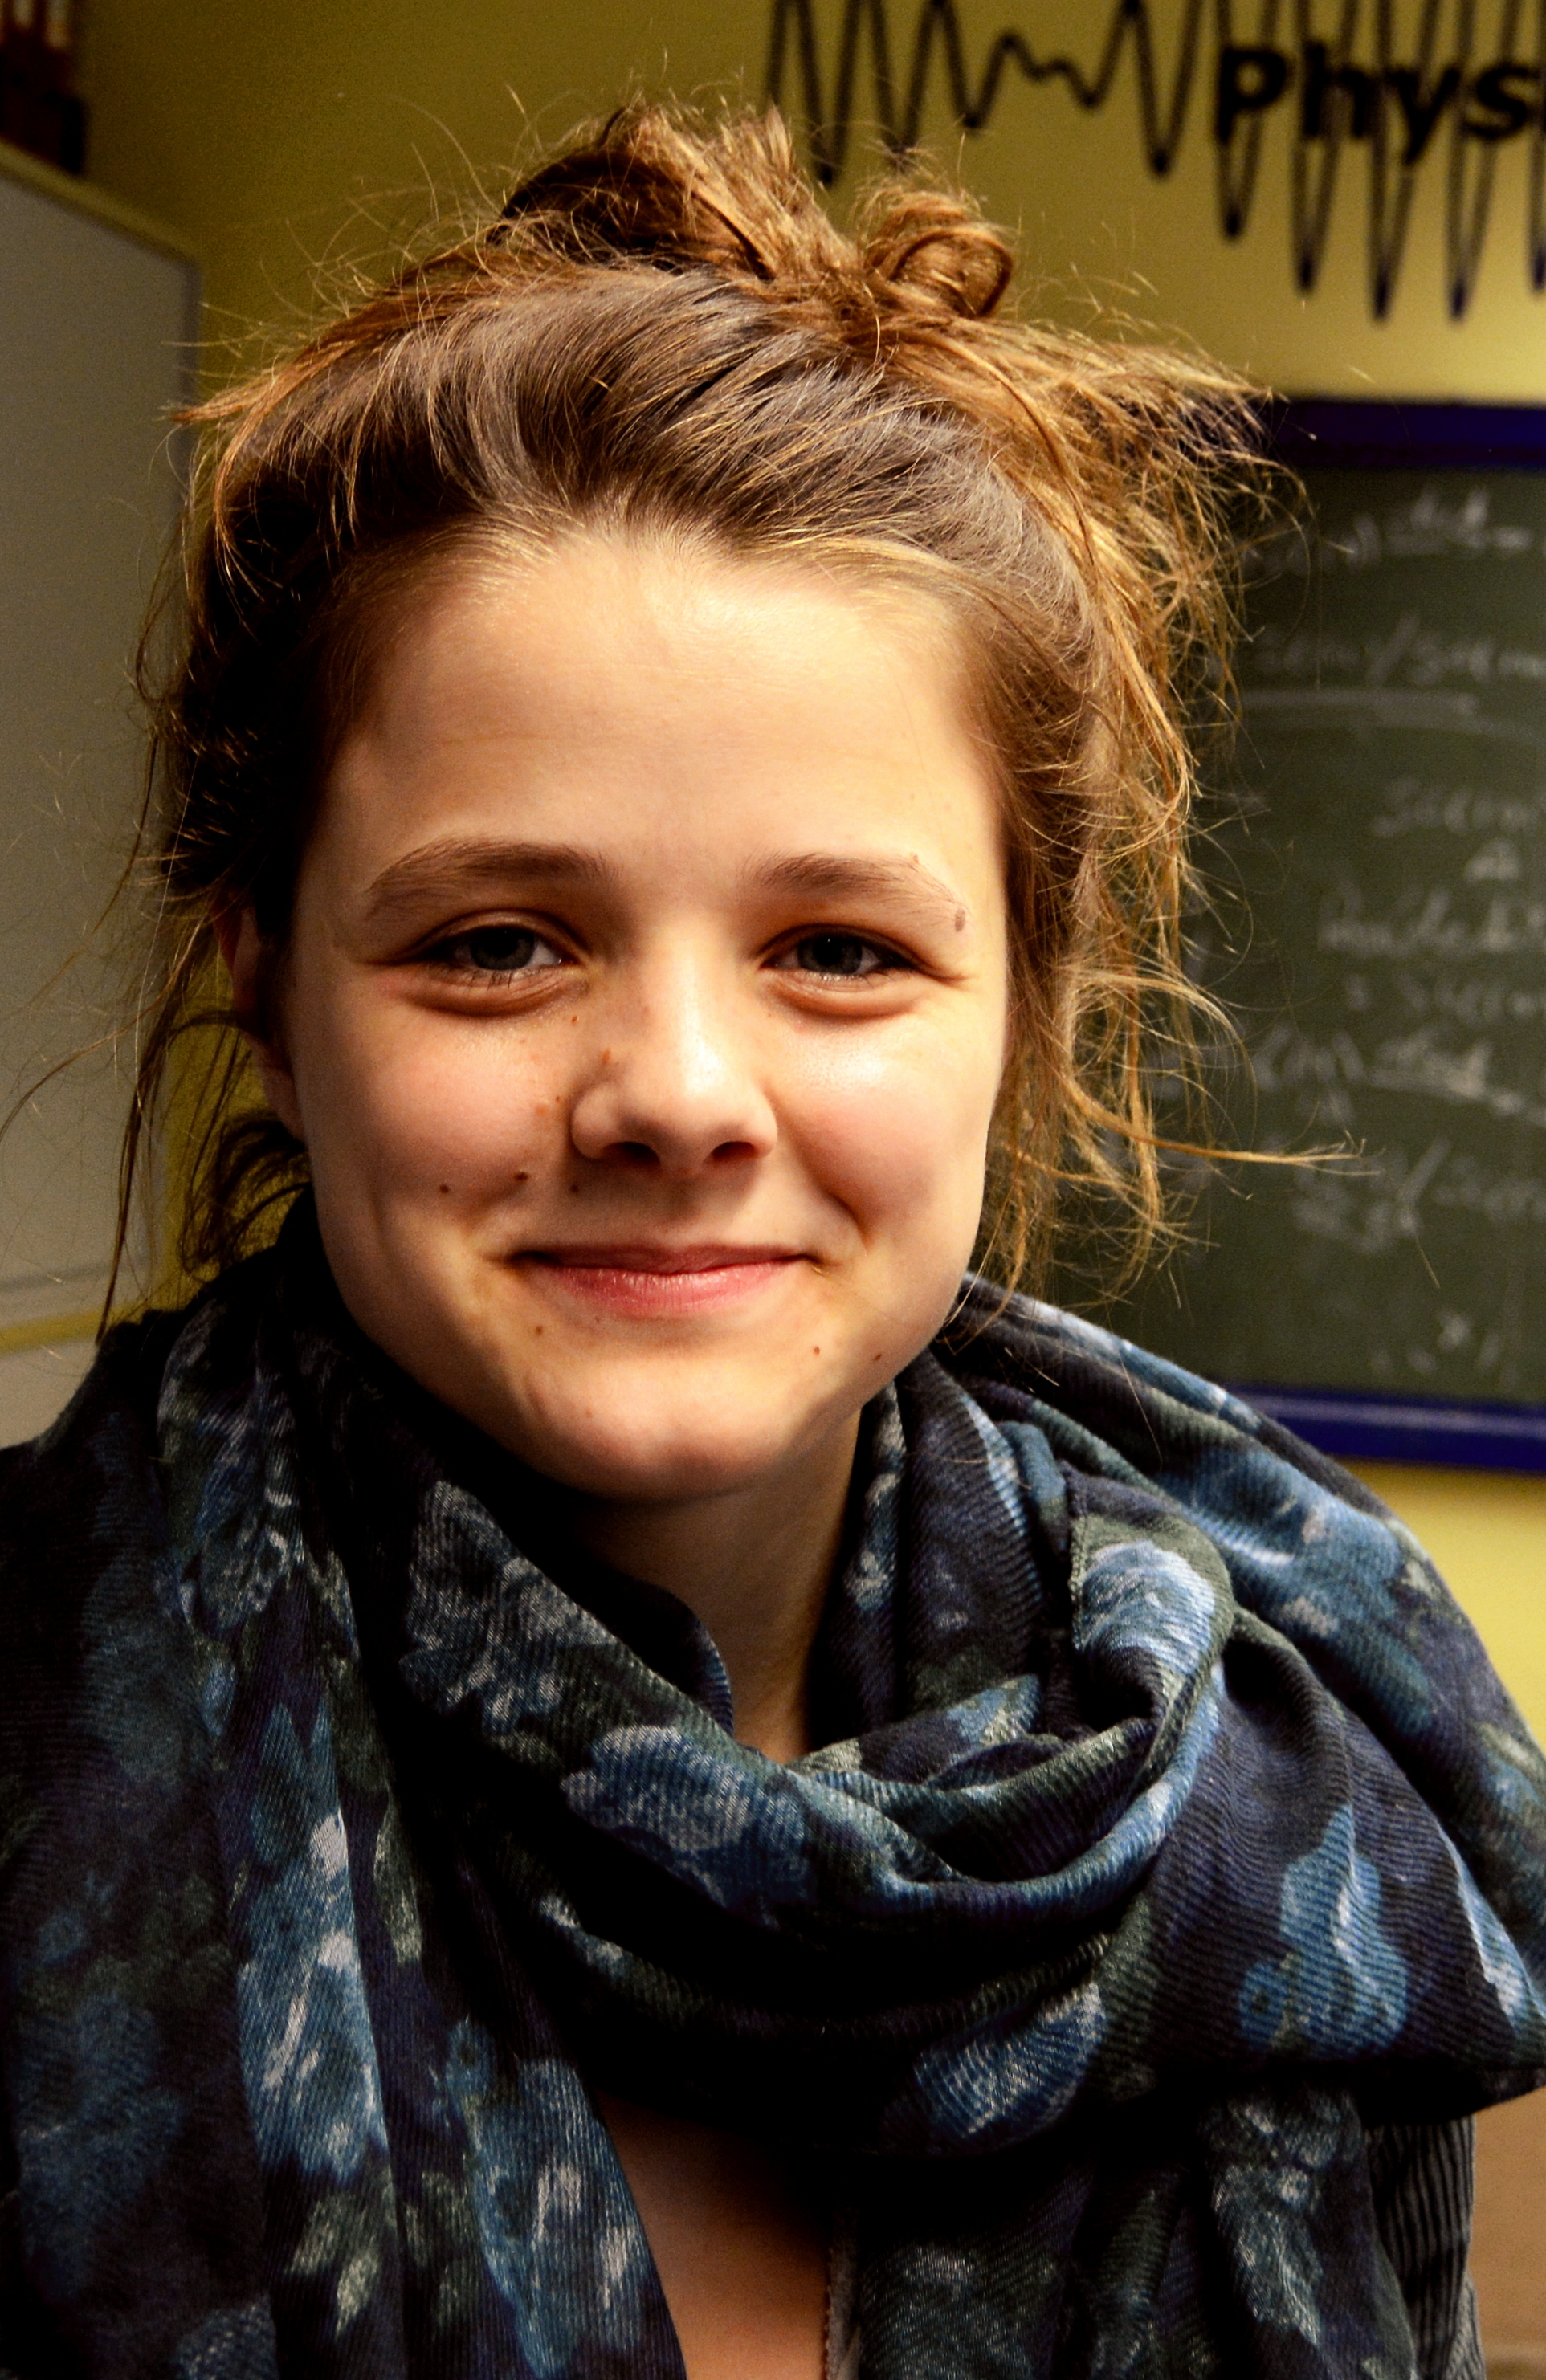
\includegraphics[width=\fibelstdlen]{res/vorstellungsfotos/pia_petrak_cropped.jpg}
	\end{wrapfigure}
}
{Hi, ich bin Pia, noch so gerade 21, und jetzt im ersten Mastersemester. Ich kümmere mich um den Bama-Tag. Da können alle Arbeitsgruppen Bachelor- und Masterarbeitsthemen vorstellen...Ansonsten will ich eigentlich nur noch los werden:
	Viel Spaß, vor allem in der O-Woche und hört bloß nicht auf mit Physik!
}

\fibelvorstellung{
	\begin{wrapfigure}{r}{0cm}
		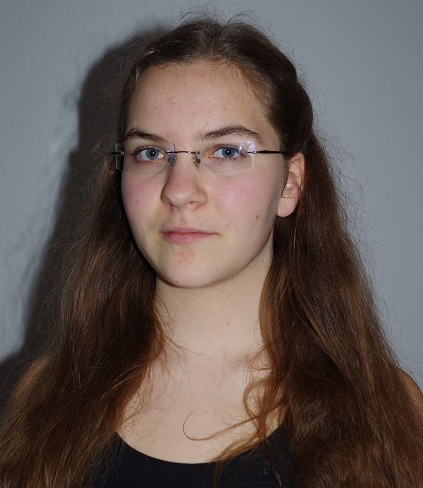
\includegraphics[width=\fibelstdlen]{res/vorstellungsfotos/andrea_garner_cropped}
	\end{wrapfigure}
}
{Hallo, ich bin Andrea und studiere seit dem WS 2016 Physik und Musik (2FB). Sollten ihr Fragen in Sachen Lehramt haben könnt ihr mich gerne ansprechen :)
	\vspace{\baselineskip}
}

\fibelvorstellung{
	\begin{wrapfigure}{l}{0cm}
		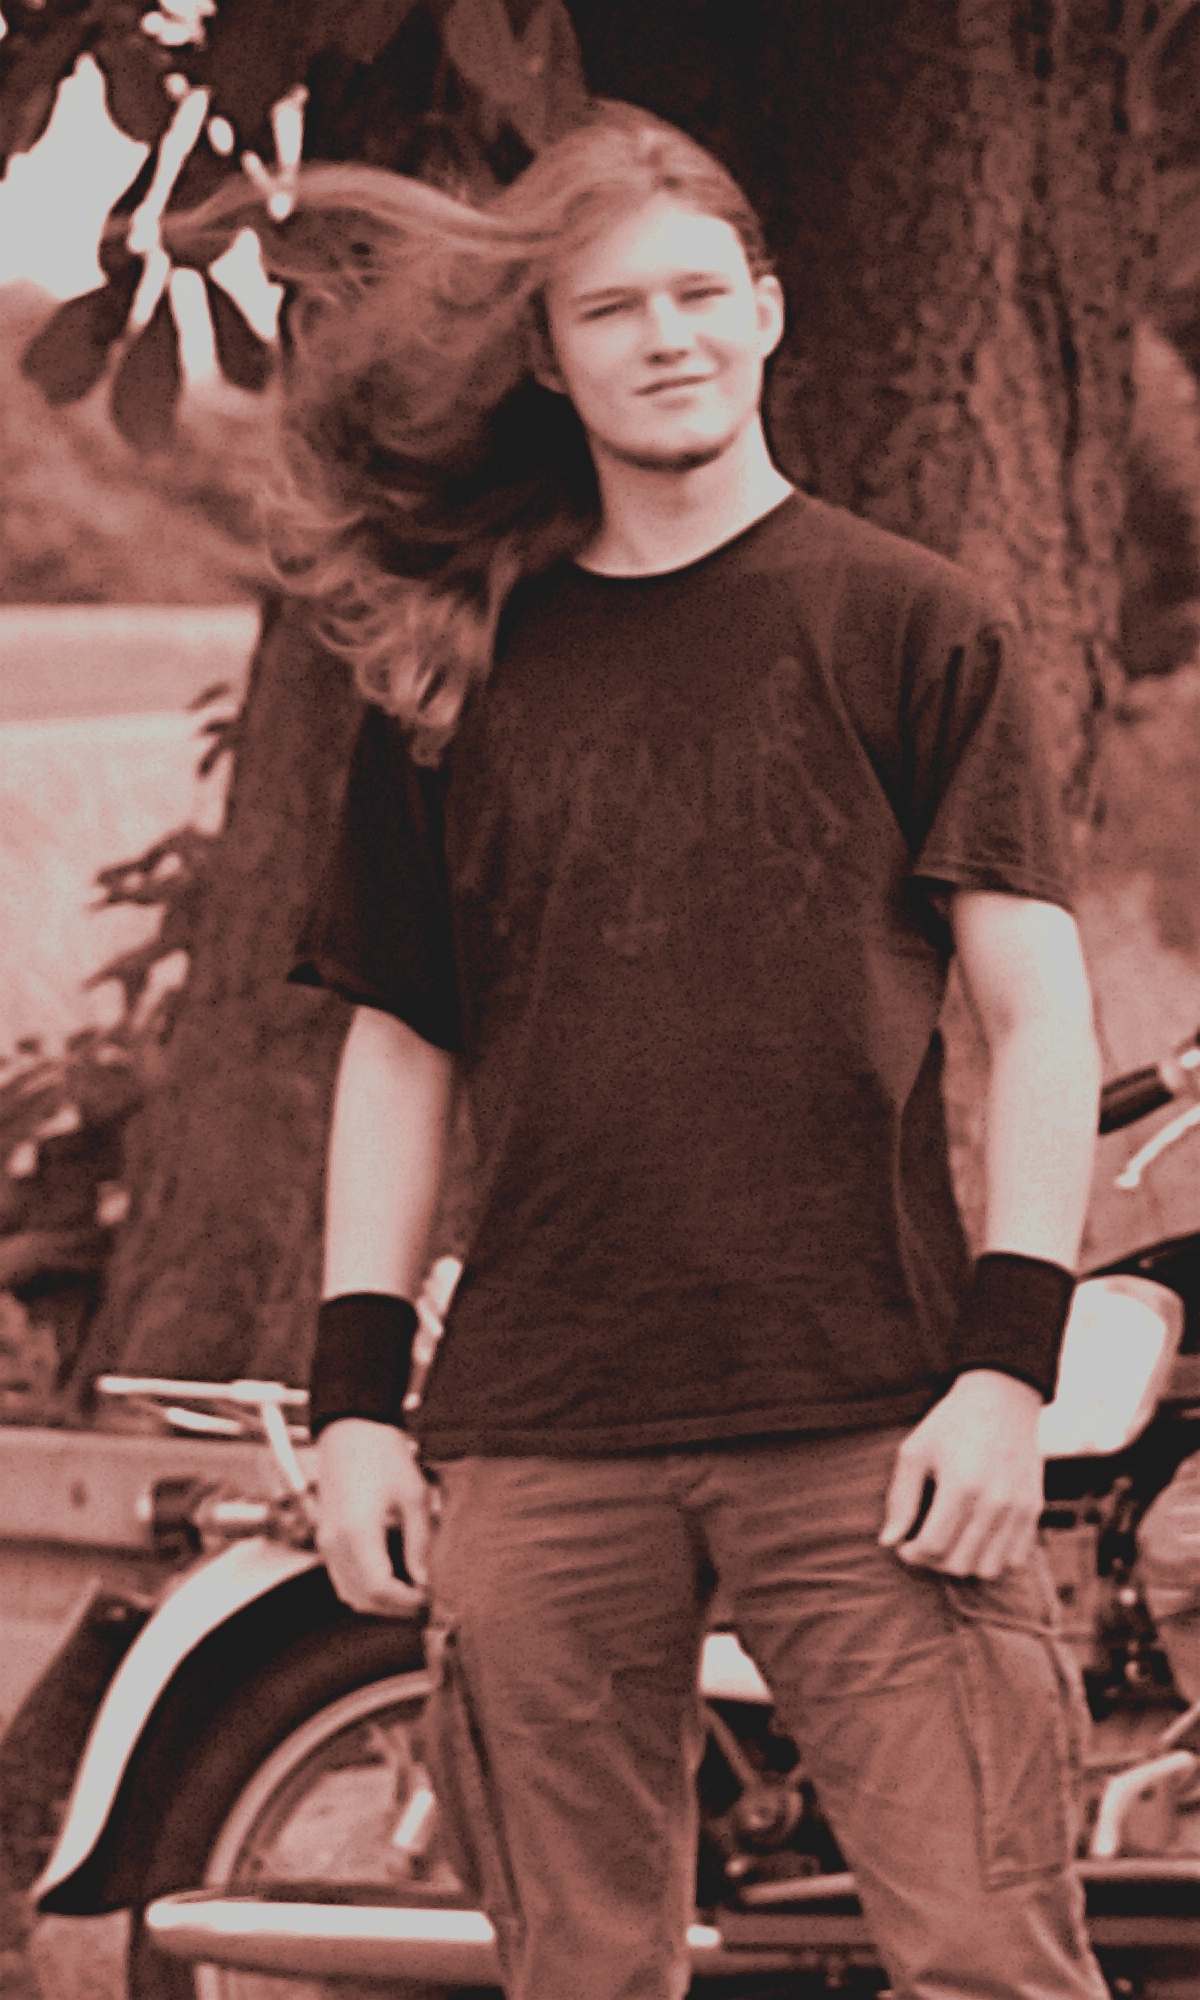
\includegraphics[width=\fibelstdlen]{res/vorstellungsfotos/jan_honermann}
	\end{wrapfigure}
}
{Hi, ich bin Jan und sitze gerade an meiner Masterarbeit. Falls ihr Fragen habt, könnt ihr euch gerne an mich wenden, ich bin meistens netter, als ich aussehe ;)
	\vspace{\baselineskip}
}


\fibelvorstellung{
	\begin{wrapfigure}{r}{0cm}
		
\includegraphics[width=.95\fibelstdlen]{res/vorstellungsfotos/jan-phillip_topmoeller.jpg}
	\end{wrapfigure}
}
{Hi. Ich bin Jan-Phillip und im dritten Semester.
	Falls ihr Fragen zum Nebenfach Mathematik habt, könnt ihr gern zu mir kommen. Aber natürlich auch für jede andere Frage oder einfach mal so ein Gespräch, habe ich jederzeit ein offenes Ohr. Allerdings bin ich nicht so häufig in der Fachschaft anzutreffen wie manch anderer, aber scheut euch nicht, mich auch außerhalb dieser anzusprechen. 
	\vspace{\baselineskip}}

\fibelvorstellung{
	\begin{wrapfigure}{l}{0cm}
		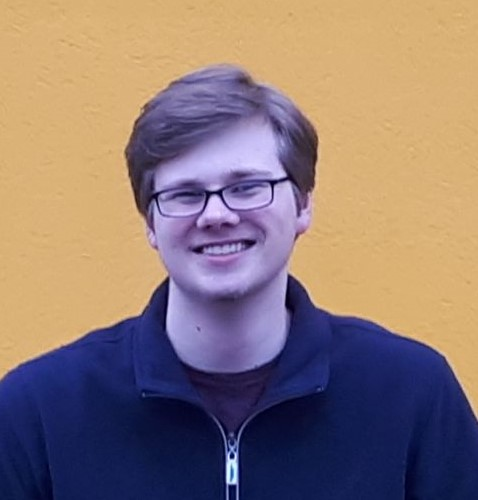
\includegraphics[width=3.2cm]{res/vorstellungsfotos/joern_sieveneck.jpg}
	\end{wrapfigure}
}
{Hi, ich bin Jörn und bin mittlerweile im 5. Semester Physik
	aber ich bin erst seit einem Semester in der Fachschaft Aktiv.
	Trotzdem könnt ihr euch bei Fragen immer gerne an mich wenden.}

\columnbreak

\fibelvorstellung{
	\begin{wrapfigure}{r}{0cm}
		\includegraphics[width=\fibelstdlen]{res/vorstellungsfotos/tarek_nicolin.JPG}
	\end{wrapfigure}
}
{Hi,
	ich bin Tarek und studiere jetzt im 5,-ten Semester. Dennoch werde ich euch ab und zu mal in Physik 1 besuchen. \\
	Wünsche euch nen guten Start und haltet durch.}


\fibelvorstellung{
	\begin{wrapfigure}{l}{0cm}
		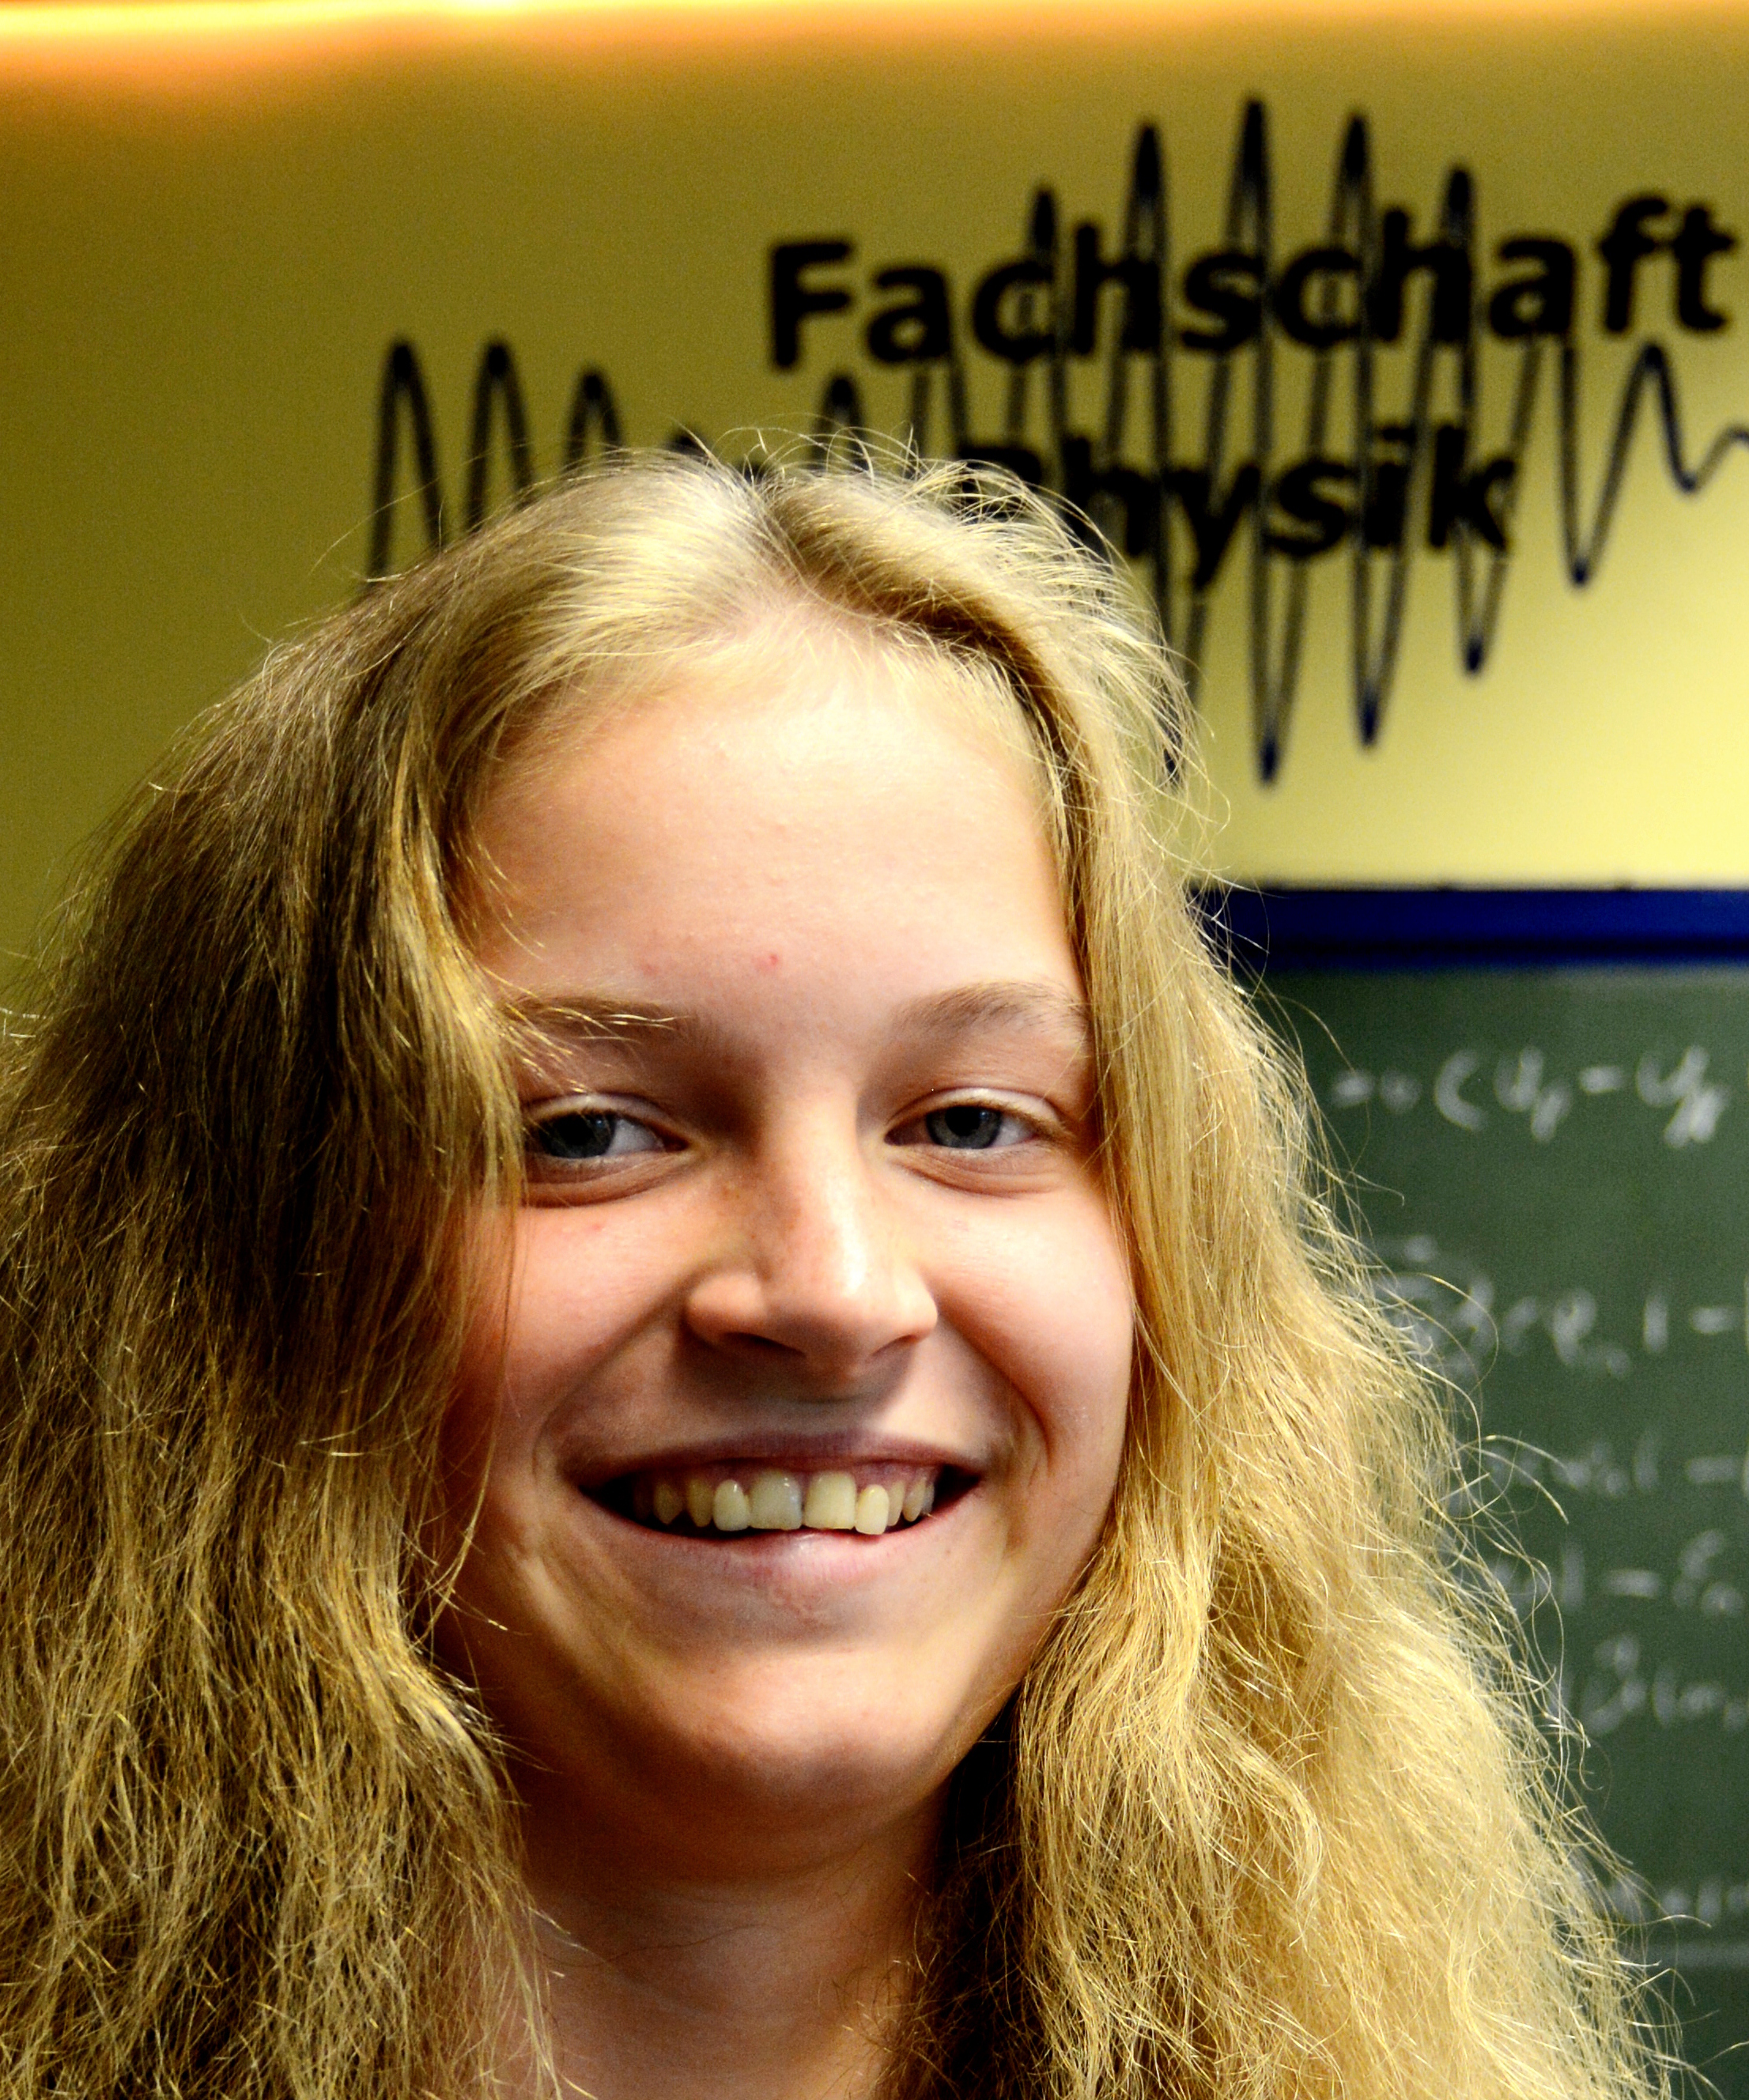
\includegraphics[width=\fibelstdlen]{res/vorstellungsfotos/johanna_jakob_cropped.jpg}
	\end{wrapfigure}
}
{Moin! Ich bin Johanna und fange in diesem Semester mit dem ersten Masterjahr an. In der Fachschaft bin ich von Anfang an dabei und als Finanzer tätig.
}
	
\fibelvorstellung{
	\begin{wrapfigure}{r}{0cm}
		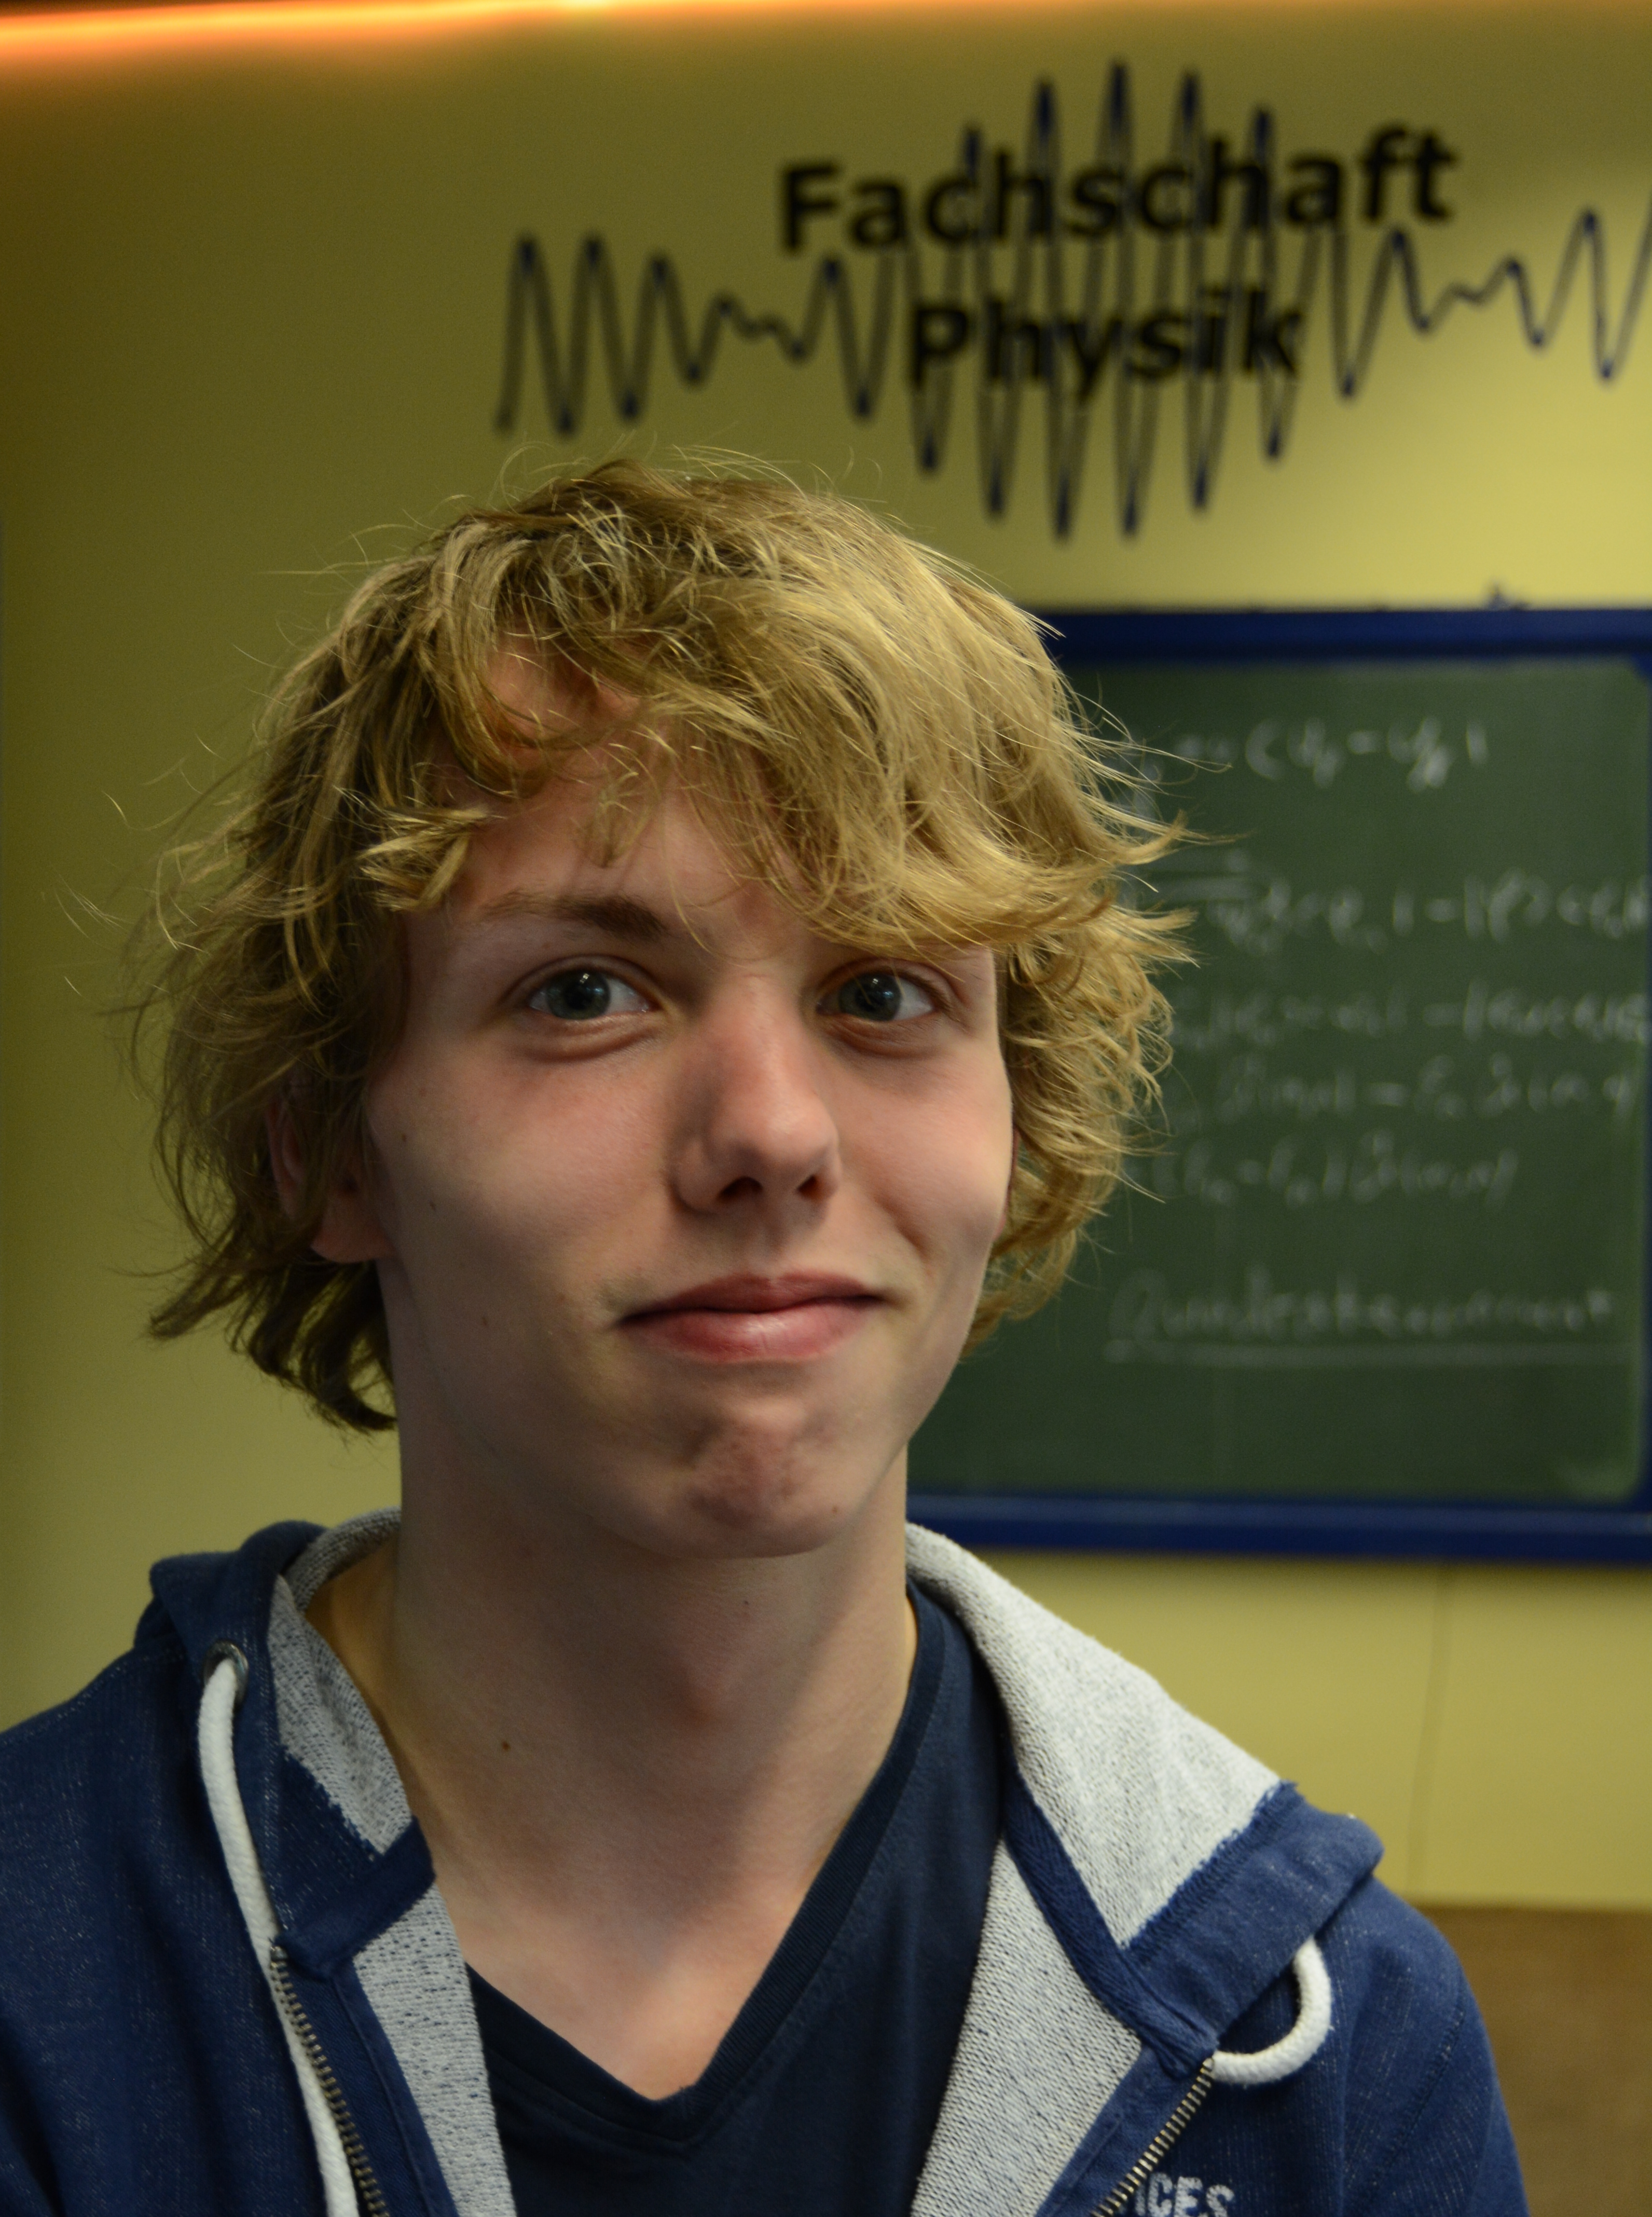
\includegraphics[width=\fibelstdlen]{res/vorstellungsfotos/marius_willer_cropped.jpg}
	\end{wrapfigure}
}
{Hi, ich bin Marius und heiße euch auch herzlich willkommen hier in Münster. Wenn ihr die Stadt noch nicht kennt, dann freut euch darauf, sie kennenzulernen. Das Studium wird zwar hart, aber lasst euch trotzdem nicht die Freude dran nehmen. ¡ Mucha suerte !}


\fibelvorstellung{
	\begin{wrapfigure}{l}{0cm}
		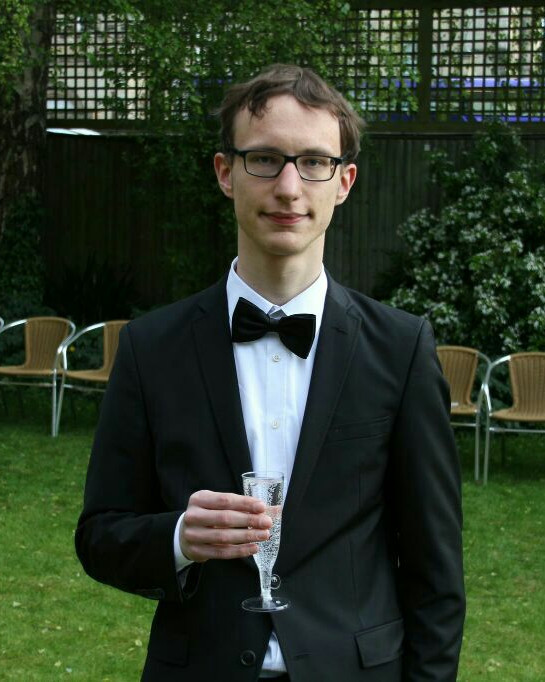
\includegraphics[width=\fibelstdlen]{res/vorstellungsfotos/michael_te_vrugt_cropped}
	\end{wrapfigure}
}
{Hi, ich bin Michael, studiere im 9. Semester Physik und Philosophie und beginne gerade mit meiner Masterarbeit. In der Fachschaft bin ich momentan Vorsitzender und Mitglied verschiedener Gremien, außerdem bin ich u.A. für die Facebook-Seite zuständig. Bei Fragen zu Philosophie, einem Doppelstudium, Auslandsjahr oder Stipendium - oder natürlich auch allem anderen - seid ihr bei mir genau richtig. Ich wünsche euch schon einmal viel Spaß in diesem tollen Studiengang!}

\fibelvorstellung{
	\begin{wrapfigure}{r}{0cm}
		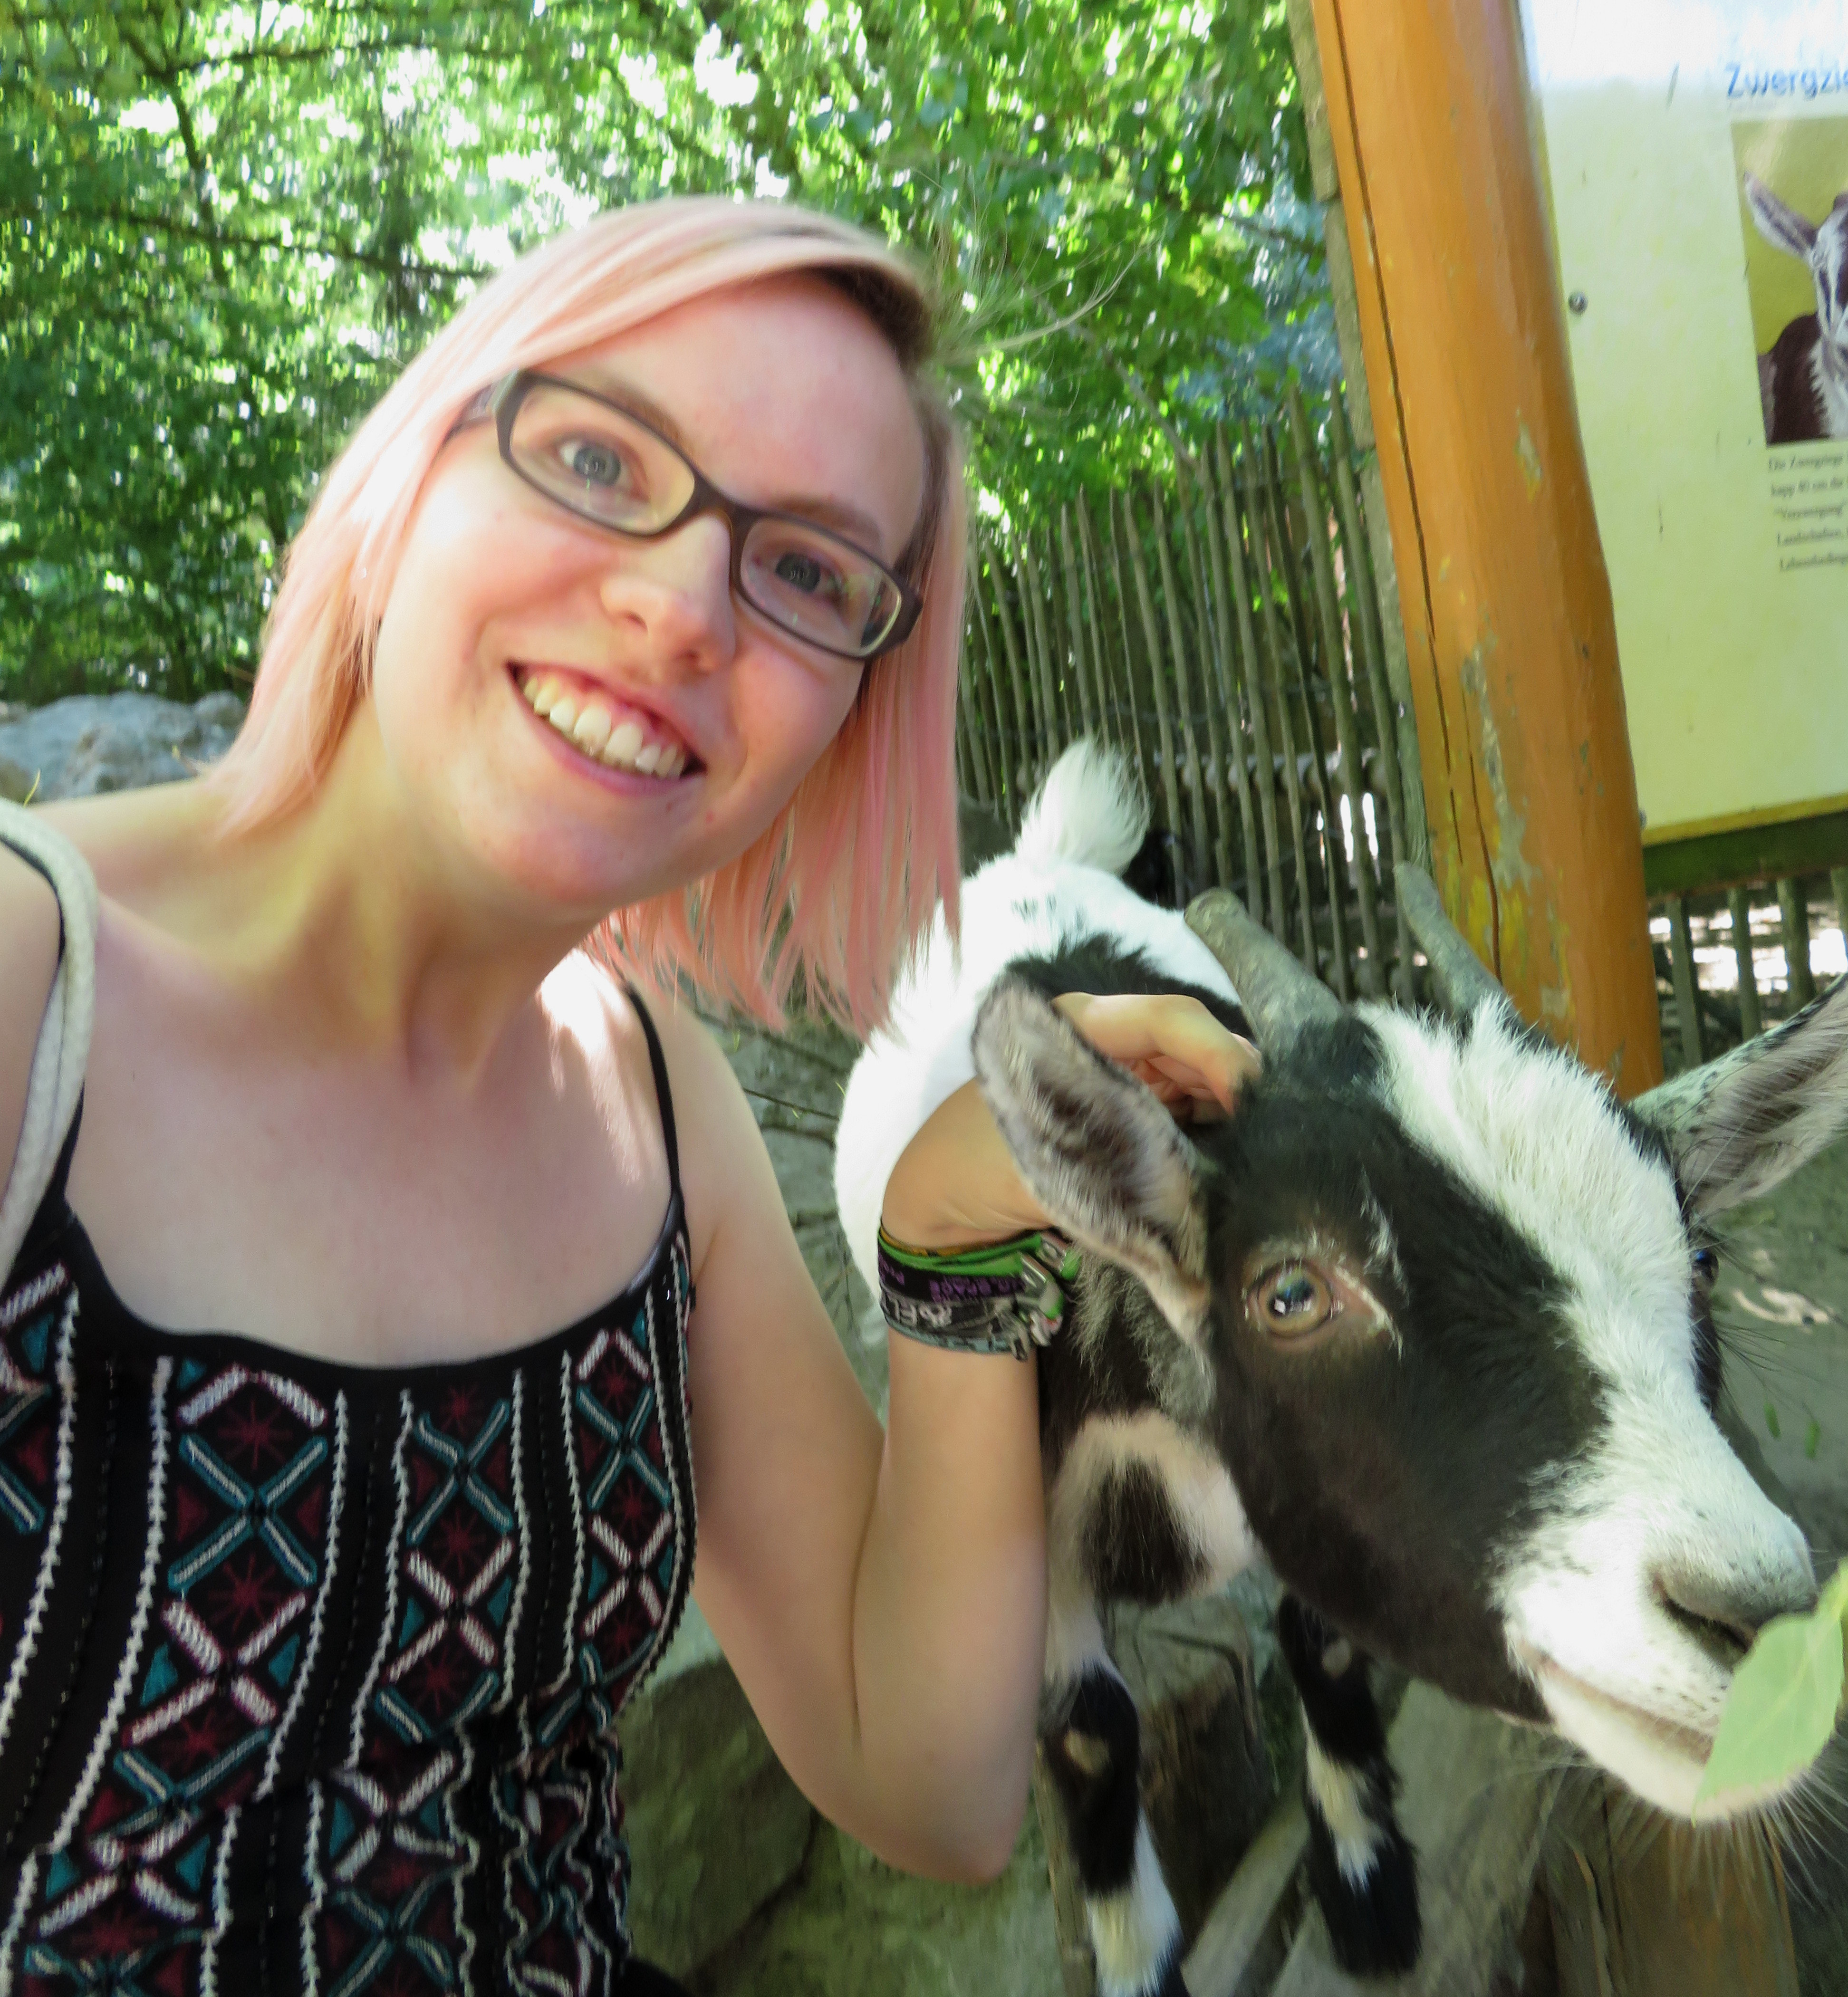
\includegraphics[width=\fibelstdlen]{res/vorstellungsfotos/miriam_neumann_cropped.jpg}
	\end{wrapfigure}
}
{Hey, ich bin Miri, 22 und gerade mitten in meinem Master. Bei einem Tee (oder Bier ;)) könnt ihr mich gerne über das Studium oder die Stadt ausfragen. Auch falls ihr sonst etwas wissen wollt, Hilfe braucht oder einfach nur quatschen wollt, seit ihr willkommen! Man erkennt mich am rosa Haar (oder anderen Farbexperimenten) :-)}







	

	


%
% \begin{center}
% 	
\includegraphics[width=\columnwidth]{res/fsphys_logo.pdf}
% \end{center}
%
%
%

%\vspace{6ex}
%
%\fibelvorstellung{
%	\begin{wrapfigure}{r}{0cm}
%		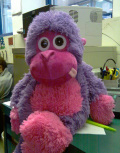
\includegraphics[width=\fibelstdlen]{res/vorstellungsfotos/fritz.png}
%	\end{wrapfigure}
%}
%{Hallo, ich bin Fritz und bin neu in der Fachschaft Physik.
%Die Mannschaft hier ist echt genial aufgestellt, sodass es richtigen Spaß macht, ein aktiver Teil der Universität Münster zu sein.
%Ich kann dir nur empfehlen: Mach' mit und verändere die Uni!}
\end{multicols*}

